\documentclass{beamer}

% language
%\usepackage[ngerman]{babel}   % include for German presentations

% font encryption
\usepackage[T1]{fontenc}
\usepackage[utf8]{inputenc}
%\usepackage[latin1]{inputenc}

% styles
\usepackage{multimedia}
\usepackage{tabularx}

% figures
\usepackage{natbib} 
\usepackage{subfig}
\usepackage{color} 
\usepackage{graphicx}
\usepackage{graphics}
\usepackage{epsfig}

% necessary packages for layout
\usepackage{beamerthemesplit}
\usepackage{watermark}
\usepackage{helvet} % fonttype

% math package
\usepackage{amsmath}
\usepackage{amsfonts}
\usepackage{mathtools}
\everymath{\displaystyle} % avoids smaller math fonts of fractions

%tikz
\usepackage{tikz,pgfplots}
\usetikzlibrary{calc,intersections,through,backgrounds,decorations.text,patterns}
\usetikzlibrary{decorations.pathreplacing,decorations.markings}


\usepackage{amsmath}
\usepackage{amsfonts}
\usepackage{amssymb}
\usepackage{tikz}
\usetikzlibrary{shapes}
\usetikzlibrary{arrows}
\usetikzlibrary{positioning}
\usetikzlibrary{decorations.markings}
\usepackage{bm}
\usepackage{makeidx}
\usepackage{graphicx}
\usepackage{caption}
\usepackage{subfig}
\usepackage{siunitx}
\usepackage{accents}
\newcommand*{\dt}[1]{%
	\accentset{\mbox{\large\bfseries .}}{#1}}
\usepackage{float}
%\usepackage[backend= bibtex,sorting=none,citestyle=numeric,bibstyle=numeric]{biblatex}
%\usepackage[left=2cm,right=2cm,top=2cm,bottom=2cm]{geometry}
\usepackage[absolute,overlay]{textpos}

%\usepackage{pstricks}
%\usepackage{pst-fill,pst-grad}
%\usepackage{pst-text}
%\usepackage{pst-uml}
\usepackage{pdfpages}
%\usepgfplotslibrary{external}
%\tikzexternalize
%\tikzsetexternalprefix{external_figs/}
\pgfplotsset{compat=newest}
%% the following commands are needed for some matlab2tikz features
\usetikzlibrary{plotmarks}
\usetikzlibrary{arrows.meta}
%\usepgfplotslibrary{patchplots}
\usepackage{grffile}

\usepackage{tabularx}

\usetikzlibrary{matrix,positioning,decorations.pathreplacing}
\DeclareMathOperator{\Mcol}{col}
\DeclareMathOperator{\Mrow}{row}
\DeclareMathOperator{\Mnull}{null}
%\usepackage[latin1]{inputenc}
\usetikzlibrary{shapes,arrows}
%%\usepackage[active,tightpage,pdftex]{preview}
%\usepackage{mathtools}
%\usepackage{pgfplots}
%\usepackage{siunitx}
%
%\usepackage{tikz}
\usetikzlibrary{shapes}
\usetikzlibrary{calc}
\usepackage{setspace}% http://ctan.org/pkg/setspace

\usepackage{animate}
\usepackage{media9}
\usepackage[]{algorithm2e}
\usepackage{amsmath,amsthm,amstext,amssymb}
%\usepackage[export]{adjustbox}
\usepackage{multimedia}
\usepackage{animate}
\usepackage{xmpmulti}

% font definitions
\usefonttheme{professionalfonts}
\setbeamerfont{title}{series=\bfseries}
\setbeamerfont{subtitle}{series=\mdseries}
\setbeamerfont{frametitle}{series=\mdseries}
\setbeamerfont{footline}{series=\mdseries}%, size=\scriptsize}
\linespread{1.2}

% Color definitions
\definecolor{luhBlue}{RGB}{0,80,155}
\definecolor{luhBlue40}{RGB}{153,185,216}
\definecolor{luhBlue20}{RGB}{204,220,235}
\definecolor{luhGreen}{RGB}{200,211,23}
\definecolor{darkGray}{RGB}{153,153,153}
\definecolor{lightGray}{RGB}{204,204,204}

\setbeamercolor{title}{fg=luhBlue}
\setbeamercolor{subtitle}{fg=luhBlue40}
\setbeamercolor{titlelike}{fg=luhBlue,parent=structure}
\setbeamercolor{titlelike}{fg=luhBlue,bg=}
\setbeamercolor{normal text}{fg=black}
\setbeamercolor{alerted text}{fg=luhGreen}
\setbeamercolor{example text}{fg=luhBlue20}
\setbeamercolor{structure}{fg=black}


\setbeamercolor{itemize item}{fg=darkGray}
\setbeamercolor{itemize subitem}{fg=darkGray}
\setbeamercolor{itemize subsubitem}{fg=darkGray}

\setbeamercolor{item projected}{fg=white,bg=darkGray}
\setbeamercolor{enumerate subitem}{fg=darkGray}
\setbeamercolor{enumerate subsubitem}{fg=darkGray}

%\setbeamertemplate{itemize items}[ball]
%\setbeamertemplate{items}[ball]

% Blocks
\setbeamercolor{block body}{fg=black,bg=white}
\setbeamercolor{block body alerted}{fg=black,bg=white}
\setbeamercolor{block body example}{fg=black,bg=white}
\setbeamercolor{block title}{fg=white,bg=luhBlue}
\setbeamercolor{block title alerted}{use={normal text,alerted text},fg=black,bg=luhGreen}
\setbeamercolor{block title example}{use={normal text,example text},fg=black,bg=luhBlue40}

% Sidebar
% \setbeamercolor{palette sidebar primary}{fg=white}
% \setbeamercolor{palette sidebar secondary}{fg=luhBlue20}
% \setbeamercolor{palette sidebar tertiary}{fg=white}
% \setbeamercolor{palette sidebar quaternary}{fg=luhBlue}
% \setbeamercolor{sidebar}{bg=luhBlue40}
% \setbeamercolor{section in sidebar}{fg=luhBlue}
% \setbeamercolor{section in sidebar shaded}{fg= luhBlue20}
% \setbeamercolor{subsection in sidebar}{use=section in sidebar, fg=section in sidebar.fg}
% \setbeamercolor{subsection in sidebar shaded}{use=section in sidebar shaded, fg=section in sidebar shaded.fg}

% Layout
\useinnertheme{rectangles}
%\useoutertheme{miniframes}
\beamertemplatenavigationsymbolsempty
%\setbeamercovered{transparent} % hidden content is transparent
\setbeamercovered{invisible} % hidden content is invisible
\setbeamercolor{section number projected}{bg=darkGray,fg=white}
\setbeamercolor{subsection number projected}{bg=darkGray,fg=white}
\setbeamersize{sidebar width left=2px}

% headline design
\setbeamertemplate{headline}{
\begin{picture}(0,-10)(-230,30)
\put(15,6){\includegraphics[height=20px]{ens.png}}
\end{picture}
\begin{picture}(0,-10)(-275,30)
\put(14,6){\includegraphics[height=20px]{IMAGES/Logos_intern/luh.eps}}
\end{picture}
}

%\setbeamerfont{footline}{size=\fontsize{10}{12}\selectfont}

%\addtobeamertemplate{frametitle}{\vskip1.8ex \hspace*{0.2cm}}{}

%\addtobeamertemplate{framesubtitle}{\vskip0.8ex \hspace*{0.2cm}}{}
%\setbeamertemplate{framesubtitle}{\vskip0.5cm \hskip0.25cm \insertframesubtitle}

% extended footline starting on slide 2
\setbeamertemplate{footline}{
\color{lightGray}
\rule{\textwidth}{18px}
\begin{picture}(0,0)(0,0)
\put(41.5,0){\includegraphics[height=18px]{IMAGES/Logos_intern/ibnmlogogruen.eps}}
\end{picture}
\begin{picture}(0,0)(0,0)
\put(-2,0){\includegraphics[height=18px]{IMAGES/irtg_1627_Logo-neu2014_links.eps}}
\end{picture}
\begin{picture}(0,0)(0,0)
\put(14.5,0){\includegraphics[height=18px]{LMT.jpg}}
\end{picture}
\begin{picture}(0,0)(-275,-15)
\color{luhGreen}\rule{80px}{3px}
\end{picture}
\color{black}
\begin{picture}(0,0)(-60,-7)
\insertshortauthor\\ \insertshorttitle\\ \insertshortdate 
\end{picture}
\begin{picture}(0,0)(-346,-7)
\insertframenumber
\end{picture}
}

% sidebar design

%\setbeamersize{sidebar width left=5px}
\setbeamertemplate{sidebar canvas left}{
\hspace*{-0.72cm}
\includegraphics[height=1.2\textheight,width=14.5mm]{IMAGES/Logos_intern/Gitter_Rad_neu.eps}
}

% title page design
\setbeamertemplate{title page}{
\vspace{1cm}
\hspace*{-0.8cm}
\usebeamerfont{title}\usebeamercolor[fg]{title}\inserttitle\par
\usebeamerfont{subtitle}\usebeamercolor[fg]{subtitle}\insertsubtitle\par
\bigskip
\begin{flushright}
\usebeamerfont{author}\usebeamercolor[fg]{normal text}\insertauthor\par
\usebeamerfont{institute}\insertinstitute\par
\usebeamerfont{date}\insertdate\par
\end{flushright}
\hspace*{-0.8cm}
\begin{picture}(0,0)(0,40)
\usebeamercolor[fg]{titlegraphic}\inserttitlegraphic
\end{picture}
}

\newcommand{\specialTitleDesign}{

% colored mesh on title page

\setbeamertemplate{sidebar canvas left}{
\hspace*{-0.72cm}
\vspace*{-0.5cm}
\includegraphics[height=1.2\textheight,width=14.3mm]{IMAGES/Logos_intern/Gitter_Rad_Gruen.eps}
}

% larger header on title page
\setbeamertemplate{headline}{
\begin{picture}(0,-10)(-190,30)
\put(25,-1){\includegraphics[width=58px]{ens.png}}
\end{picture}
\begin{picture}(0,-10)(-275,30)
\put(0,0){\includegraphics[width=80px]{IMAGES/Logos_intern/luh.eps}}
\end{picture}	
	
%\begin{picture}(0,-10)(-50,50)
%\put(0,3){\includegraphics[width=120px]{ens.png}}
%%\put(0,3){\includegraphics[width=30px]{IMAGES/irtg_1627_Logo-neu2014_links.eps}}
%%\put(33,17){\scalebox{.85}{ViVaCE `` Virtual Materials and their}}
%%\put(33,10){\scalebox{.85}{Validation: German-French School of }}
%%\put(33,3){\scalebox{.85}{Computational Engineering'' - IRTG 1627 }}
%\end{picture}	
%\begin{picture}(0,0)(-215,48)
%\includegraphics[width=140px]{IMAGES/Logos_intern/luh.eps}
%\end{picture}
}

% clean footline on title page
\setbeamertemplate{footline}{
\color{lightGray}
\rule{\textwidth}{18px}
\begin{picture}(0,0)(0,0)
\put(41.5,0){\includegraphics[height=18px]{IMAGES/Logos_intern/ibnmlogogruen.eps}}
\end{picture}
\begin{picture}(0,0)(0,0)
\put(-2,0){\includegraphics[height=18px]{IMAGES/irtg_1627_Logo-neu2014_links.eps}}
\end{picture}
\begin{picture}(0,0)(0,0)
\put(14.5,0){\includegraphics[height=18px]{LMT.jpg}}
\end{picture}
%\begin{picture}(0,0)(0,0)
%\put(20,0){\includegraphics[height=18px]{IMAGES/dfg_logo.eps}}
%\end{picture}
}
\addtocounter{framenumber}{-1} % set title page to count 0
}

\newcommand{\dfgFunding}{
	\begin{figure}
\begin{flushright}
Funded by:\\
\includegraphics[width=0.15\textwidth]{IMAGES/Logos_extern/dfg_blue.eps}
\end{flushright}
\end{figure}
}

\newcommand{\contiFunding}{
	\begin{figure}
%	Funded by:\\[-0.3cm]
	\begin{flushright}
		\setlength{\unitlength}{\textwidth}
		\begin{picture}(0.47,0)
		\includegraphics[height=18px]{IMAGES/dfg_logo.eps}
		\end{picture}
%		\\[-0.5cm]
%		{\flushleft \tiny \color{blue} IRTG 1627}
	\end{flushright}\vspace*{-0.3cm}
	\qquad \qquad \quad {\scriptsize IRTG-1627}
\end{figure}
}

\setbeamertemplate{frametitle}{
\vskip2ex \hspace*{-0.4cm} {\insertframetitle} \\[-0.2cm]
\hskip0.15cm  {\small \insertframesubtitle}\\[-0.6cm] }


\newcommand{\ltab}{\raggedright\arraybackslash} % Tabellenabschnitt linksbündig
\newcommand{\ctab}{\centering\arraybackslash} % Tabellenabschnitt zentriert
\newcommand{\rtab}{\raggedleft\arraybackslash} % Tabellenabschnitt rechtsbündig

% \newcommand{\ul}[1]{\underline{#1}}
% \newcommand{\ull}[1]{\uline{\raisebox{-0.05em}{\uline{\raisebox{0.05em}{\ensuremath{#1}}}}}}
\newcommand{\ul}[1]{\underline{#1}}
\newcommand{\ull}[1]{\ul{\ul{#1}}}
\makeatletter
\definecolor{Sblueaa}{cmyk}{1,0.6,0,0}
\definecolor{Sbluea}{cmyk}{1,0.4,0,0}
\definecolor{Sblueb}{cmyk}{0.7,0.2,0,0}
\definecolor{Sbluec}{cmyk}{0.5,0.1,0,0}
\definecolor{Sblued}{cmyk}{0.3,0.05,0,0}
\definecolor{Sbluee}{cmyk}{0.15,0.04,0,0}
\definecolor{Svbluea}{cmyk}{0.9,0.6,0,0}
\definecolor{Svblueb}{cmyk}{0.68,0.4,0,0}
\definecolor{Svbluec}{cmyk}{0.45,0.26,0,0}
\definecolor{Svblued}{cmyk}{0.27,0.12,0,0}
\definecolor{Sblacka}{cmyk}{0.5,0.2,0.2,0.85}
\definecolor{Sblackb}{cmyk}{0.35,0.14,0.14,0.6}
\definecolor{Sblackc}{cmyk}{0.25,0.1,0.1,0.43}
\definecolor{Sblackd}{cmyk}{0.15,0.06,0.06,0.26}
\definecolor{Sblacke}{rgb}{0.827451,0.8509804,0.8627451}
\colorlet{Sblackf}{Sblacke!70!white}

\definecolor{Syellow}{cmyk}{0,0.1,1,0}
\definecolor{Sorange}{cmyk}{0,0.7,1,0}
\definecolor{Sred}{cmyk}{0,1,1,0}
\colorlet{Slred}{Sred!40!white}
\definecolor{Spink}{cmyk}{0,1,0,0}
\definecolor{Spurple}{cmyk}{0.6,1,0,0}
\definecolor{Scyan}{cmyk}{1,0,0.4,0}
\definecolor{Sgreen}{cmyk}{0.5,0,1,0}
% \definecolor{S}{cmyk}{}

\newcommand{\cSblueaa}{\color{Sblueaa}}
\newcommand{\cSbluea}{\color{Sbluea}}
\newcommand{\cSblueb}{\color{Sblueb}}
\newcommand{\cSbluec}{\color{Sbluec}}
\newcommand{\cSblued}{\color{Sblued}}
\newcommand{\cSbluee}{\color{Sbluee}}
\newcommand{\cSvbluea}{\color{Svbluea}}
\newcommand{\cSvblueb}{\color{Svblueb}}
\newcommand{\cSvbluec}{\color{Svbluec}}
\newcommand{\cSvblued}{\color{Svblued}}
\newcommand{\cSblacka}{\color{Sblacka}}
\newcommand{\cSblackb}{\color{Sblackb}}
\newcommand{\cSblackc}{\color{Sblackc}}
\newcommand{\cSblackd}{\color{Sblackd}}
\newcommand{\cSblacke}{\color{Sblacke}}
\newcommand{\cSblackf}{\color{Sblackf}}
\newcommand{\cSyellow}{\color{Syellow}}
\newcommand{\cSorange}{\color{Sorange}}
\newcommand{\cSred}{\color{Sred}}
\newcommand{\cSdred}{\color{Sred!50!black}}
\newcommand{\cSlred}{\color{Sred!50!white}}
\newcommand{\cSpink}{\color{Spink}}
\newcommand{\cSpurple}{\color{Spurple}}
\newcommand{\cScyan}{\color{Scyan}}
\newcommand{\cSgreen}{\color{Sgreen}}
\newcommand{\cSdgreen}{\color{Sgreen!50!black}}
\newcommand{\mcode}[1]{{\cSblueb \texttt{#1}}}

\newcommand{\Sbfit}[1]{{\cSbluea\it\bfseries{#1}}}
\newcommand{\Sbf}[1]{{\cSbluea\bf #1}}
\newcommand{\Sit}[1]{{\cSbluea\it #1}}
\newcommand{\Sbfcyan}[1]{{\cScyan\bf #1}}
\newcommand{\Sbfitcyan}[1]{{\cScyan\it\bfseries #1}}
\newcommand{\Sitcyan}[1]{{\cScyan\it #1}}
\newcommand{\Sbfgreen}[1]{{\cSgreen\bf #1}}
\newcommand{\Sbfitgreen}[1]{{\cSgreen\it\bfseries #1}}
\newcommand{\Sitgreen}[1]{{\cSgreen\it #1}}
\newcommand{\Sbfred}[1]{{\cSred\bf #1}}
\newcommand{\Sbfitred}[1]{{\cSred\it\bfseries #1}}
\newcommand{\Sitred}[1]{{\cSred\it #1}}
\newcommand{\Sbfpink}[1]{{\cSpink\bf #1}}
\newcommand{\Sbfitpink}[1]{{\cSpink\it\bfseries #1}}
\newcommand{\Sitpink}[1]{{\cSpink\it #1}}
\newcommand{\Sbfpurple}[1]{{\cSpurple\bf #1}}
\newcommand{\Sbfitpurple}[1]{{\cSpurple\it\bfseries #1}}
\newcommand{\Sitpurple}[1]{{\cSpurple\it #1}}
\newcommand{\Sbfyellow}[1]{{\cSyellow\bf #1}}
\newcommand{\Sbfityellow}[1]{{\cSyellow\it\bfseries #1}}
\newcommand{\Sityellow}[1]{{\cSyellow\it #1}}
\newcommand{\Sbforange}[1]{{\cSorange\bf #1}}
\newcommand{\Sbfitorange}[1]{{\cSorange\it\bfseries #1}}
\newcommand{\Sitorange}[1]{{\cSorange\it #1}}

\setbeamercolor{cboxSblacka}{fg=white,bg=Sblacka}
\setbeamercolor{cboxSblackb}{fg=white,bg=Sblackb}
\setbeamercolor{cboxSblackc}{fg=white,bg=Sblackc}
\setbeamercolor{cboxSblackd}{fg=black,bg=Sblackd}
\setbeamercolor{cboxSblacke}{fg=black,bg=Sblacke}
\setbeamercolor{cboxSbluea}{fg=white,bg=Sbluea}
\setbeamercolor{cboxSblueb}{fg=white,bg=Sblueb}
\setbeamercolor{cboxSbluec}{fg=white,bg=Sbluec}
\setbeamercolor{cboxSblued}{fg=black,bg=Sblued}
\setbeamercolor{cboxSvbluea}{fg=white,bg=Svbluea}
\setbeamercolor{cboxSvblueb}{fg=white,bg=Svblueb}
\setbeamercolor{cboxSvbluec}{fg=white,bg=Svbluec}
\setbeamercolor{cboxSvblued}{fg=black,bg=Svblued}
\setbeamercolor{cboxSred}{fg=white,bg=Sred}
\setbeamercolor{cboxSredb}{fg=white,bg=Slred}
\setbeamercolor{cboxSorange}{fg=Sblacka,bg=Sorange}
\setbeamercolor{cboxSyellow}{fg=Sblacka,bg=Syellow}
\setbeamercolor{cboxScyan}{fg=white,bg=Scyan}
\setbeamercolor{cboxSpurple}{fg=white,bg=Spurple}
\setbeamercolor{cboxSpink}{fg=white,bg=Spink}
\setbeamercolor{cboxSgreen}{fg=black,bg=Sgreen}
%\newcommand{\sty}[1]{{\bf #1}}
\newcommand{\sty}[1]{\mbox{\boldmath $#1$}}
%\newcommand{\styy}[1]{\mbox{\boldmath $\sf #1$}}
\newcommand{\styy}[1]{{\mathbb{#1}}}
\newcommand{\z}[1]{{\tilde{#1}}}
\newcommand{\vol}[1]{\langle #1 \rangle}
\newcommand{\Vol}[1]{\left\langle #1 \right\rangle}
\renewcommand{\vec}[1]{\underline{#1}}
\newcommand{\mat}[1]{\underline{\underline{#1}}}

\newcommand{\fzero}{\sty{ 0}}
% ROMAN NUMERALS
\newcommand{\rI}{{\mathit{I}}}
\newcommand{\rII}{{\mathit{II}}}
\newcommand{\rIII}{{\mathit{III}}}
\newcommand{\rIV}{{\mathit{IV}}}
\newcommand{\rV}{{\mathit{V}}}

% Indices
\newcommand{\ta}{{}^n}
\newcommand{\tb}{{}^{n+1}}
\newcommand{\tba}{{}^{n+1}_i}
\newcommand{\tbb}{{}^{n+1}_{i+1}}
\renewcommand{\r}[2]{{#2_{\langle #1 \rangle}}}
% Operators
\newcommand{\rA}{{\rm A}}
\newcommand{\rB}{{\boldsymbol {\mathrm B}}}
\newcommand{\rC}{{\boldsymbol {\mathrm C}}}
\newcommand{\rD}{{\rm D}}
\newcommand{\rE}{{\rm E}}
\newcommand{\rF}{{\rm F}}
\newcommand{\rG}{{\rm G}}
\newcommand{\rH}{{\boldsymbol {\mathrm H}}}
\newcommand{\rHsigma}{{\boldsymbol {\mathrm H}}_{\sigma} }
% \newcommand{\rI}{{\rm I}}
\newcommand{\rJ}{{\rm J}}
\newcommand{\rK}{{\rm K}}
\newcommand{\rL}{{\rm L}}
\newcommand{\rM}{{\rm M}}
\newcommand{\rN}{{\rm N}}
\newcommand{\rO}{{\rm O}}
\newcommand{\rP}{{\rm P}}
\newcommand{\rQ}{{\rm Q}}
\newcommand{\rR}{{\rm R}}
\newcommand{\rS}{{\rm S}}
\newcommand{\rT}{{\rm T}}
\newcommand{\rU}{{\rm U}}
% \newcommand{\rV}{{\rm V}}
\newcommand{\rW}{{\rm W}}
\newcommand{\rX}{{\rm X}}
\newcommand{\rY}{{\rm Y}}
\newcommand{\rZ}{{\rm Z}}
\newcommand{\rb}{{{\mathrm b}}}
% \rm
\newcommand{\ns}{{n_{\rm s}}}
\newcommand{\nc}{{n_{\rm c}}}
\newcommand{\np}{{n_{\rm p}}}
\newcommand{\Nr}{{N_{\rm r}}}
\newcommand{\Nc}{{N_{\rm c}}}
\newcommand{\Ngp}{{N_{\rm gp}}}

% bold symbols
\newcommand{\fa}{\sty{ a}}
\newcommand{\fb}{\sty{ b}}
\newcommand{\fc}{\sty{ c}}
\newcommand{\fd}{\sty{ d}}
\newcommand{\fe}{\sty{ e}}
\newcommand{\ff}{\sty{ f}}
\newcommand{\fg}{\sty{ g}}
\newcommand{\fh}{\sty{ h}}
%\renewcommand{\fi}{\sty{ i}}
\newcommand{\fj}{\sty{ j}}
\newcommand{\fk}{\sty{ k}}
\newcommand{\fl}{\sty{ l}}
\newcommand{\fm}{\sty{ m}}
\newcommand{\fn}{\sty{ n}}
\newcommand{\fo}{\sty{ o}}
\newcommand{\fp}{\sty{ p}}
\newcommand{\fq}{\sty{ q}}
\newcommand{\fr}{\sty{ r}}
\newcommand{\fs}{\sty{ s}}
\newcommand{\ft}{\sty{ t}}
\newcommand{\fu}{\sty{ u}}
\newcommand{\fv}{\sty{ v}}
\newcommand{\fw}{\sty{ w}}
\newcommand{\fx}{\sty{ x}}
\newcommand{\fy}{\sty{ y}}
\newcommand{\fz}{\sty{ z}}

\newcommand{\fA}{\sty{ A}}
\newcommand{\fB}{\sty{ B}}
\newcommand{\fC}{\sty{ C}}
\newcommand{\fD}{\sty{ D}}
\newcommand{\fE}{\sty{ E}}
\newcommand{\fF}{\sty{ F}}
\newcommand{\fG}{\sty{ G}}
\newcommand{\fH}{\sty{ H}}
\newcommand{\fI}{\sty{ I}}
\newcommand{\fJ}{\sty{ J}}
\newcommand{\fK}{\sty{ K}}
\newcommand{\fL}{\sty{ L}}
\newcommand{\fM}{\sty{ M}}
\newcommand{\fN}{\sty{ N}}
\newcommand{\fO}{\sty{ 0}}
\newcommand{\fP}{\sty{ P}}
\newcommand{\fQ}{\sty{ Q}}
\newcommand{\fR}{\sty{ R}}
\newcommand{\fS}{\sty{ S}}
\newcommand{\fT}{\sty{ T}}
\newcommand{\fU}{\sty{ U}}
\newcommand{\fV}{\sty{ V}}
\newcommand{\fW}{\sty{ W}}
\newcommand{\fX}{\sty{ X}}
\newcommand{\fY}{\sty{ Y}}
\newcommand{\fZ}{\sty{ Z}}

\newcommand{\falpha}{\mbox{\boldmath $\alpha$}}
\newcommand{\fkappa}{\mbox{\boldmath $\kappa$}}
\newcommand{\fnu}{\mbox{\boldmath $\nu$}}
\newcommand{\fchi}{\mbox{\boldmath $\chi$}}
\newcommand{\ftau}{\mbox{\boldmath $\tau$}}
\newcommand{\fsigma}{\mbox{\boldmath $\sigma$}}
\newcommand{\flambda}{\mbox{\boldmath $\lambda$}}
\newcommand{\fmu}{\mbox{\boldmath $\mu$}}
\newcommand{\fDelta}{\mbox{\boldmath $\Delta$}}
\newcommand{\fdelta}{\mbox{\boldmath $\delta$}}
\newcommand{\fomega}{\mbox{\boldmath $\omega$}}
\newcommand{\fOmega}{\mbox{\boldmath $\Omega$}}
\newcommand{\fLambda}{\mbox{\boldmath $\Lambda$}}
\newcommand{\feta}{\mbox{\boldmath $\eta $}}
\newcommand{\fxi}{\mbox{\boldmath $\xi $}}
\newcommand{\fXi}{\mbox{\boldmath $\Xi $}}
\newcommand{\feps}{\mbox{\boldmath $\varepsilon $}}
\newcommand{\fepsp}{\feps^\pl{p}}
\newcommand{\fepse}{\feps^\pl{e}}
\newcommand{\ftheta}{\mbox{\boldmath $\theta $}}
\newcommand{\fgamma}{\mbox{\boldmath $\gamma $}}
\newcommand{\fGamma}{\mbox{\boldmath $\Gamma $}}
\newcommand{\fSigma}{\mbox{\boldmath $\Sigma $}}
\newcommand{\fPi}{\mbox{\boldmath $\Pi $}}
\newcommand{\fPhi}{\mbox{\boldmath $\Phi $}}
\newcommand{\fphi}{\mbox{\boldmath $\phi $}}
\newcommand{\fpi}{\mbox{\boldmath $\pi $}}
\newcommand{\fvarphi}{\mbox{\boldmath $\varphi $}}
\newcommand{\fpsi}{\mbox{\boldmath $\psi $}}
\newcommand{\fPsi}{\mbox{\boldmath $\Psi $}}
\newcommand{\fJota}{{\bf I}}

% Sets or 4th order tensors
\newcommand{\tC}{{\mathrm {\styy C}}}

% Sets or 2nd order tensors
\newcommand{\ffa}{\styy{ a}}
\newcommand{\ffb}{\styy{ b}}
\newcommand{\ffc}{\styy{ c}}
\newcommand{\ffd}{\styy{ d}}
\newcommand{\ffe}{\styy{ e}}
\newcommand{\fff}{\styy{ f}}
\newcommand{\ffg}{\styy{ g}}
\newcommand{\ffh}{\styy{ h}}
%\renewcommand{\fi}{\styy{ i}}
\newcommand{\ffj}{\styy{ j}}
\newcommand{\ffk}{\styy{ k}}
\newcommand{\ffl}{\styy{ l}}
\newcommand{\ffm}{\styy{ m}}
\newcommand{\ffn}{\styy{ n}}
\newcommand{\ffo}{\styy{ o}}
\newcommand{\ffp}{\styy{ p}}
\newcommand{\ffq}{\styy{ q}}
\newcommand{\ffr}{\styy{ r}}
\newcommand{\ffs}{\styy{ s}}
\newcommand{\fft}{\styy{ t}}
\newcommand{\ffu}{\styy{ u}}
\newcommand{\ffv}{\styy{ v}}
\newcommand{\ffw}{\styy{ w}}
\newcommand{\ffx}{\styy{ x}}
\newcommand{\ffy}{\styy{ y}}
\newcommand{\ffz}{\styy{ z}}

\newcommand{\ffA}{\styy{ A}}
\newcommand{\ffB}{\styy{ B}}
\newcommand{\ffC}{\styy{ C}}
\newcommand{\ffD}{\styy{ D}}
\newcommand{\ffE}{\styy{ E}}
\newcommand{\ffF}{\styy{ F}}
\newcommand{\ffG}{\styy{ G}}
\newcommand{\ffH}{\styy{ H}}
\newcommand{\ffI}{\styy{ I}}
\newcommand{\ffJ}{\styy{ J}}
\newcommand{\ffK}{\styy{ K}}
\newcommand{\ffL}{\styy{ L}}
\newcommand{\ffM}{\styy{ M}}
\newcommand{\ffN}{\styy{ N}}
\newcommand{\ffO}{\styy{ O}}
\newcommand{\ffP}{\styy{ P}}
\newcommand{\ffQ}{\styy{ Q}}
\newcommand{\ffR}{\styy{ R}}
\newcommand{\ffS}{\styy{ S}}
\newcommand{\ffT}{\styy{ T}}
\newcommand{\ffU}{\styy{ U}}
\newcommand{\ffV}{\styy{ V}}
\newcommand{\ffW}{\styy{ W}}
\newcommand{\ffX}{\styy{ X}}
\newcommand{\ffY}{\styy{ Y}}
\newcommand{\ffZ}{\styy{ Z}}

%
\newcommand{\bfa}{\bar{\sty{ a}}}
\newcommand{\bfb}{\bar{\sty{ b}}}
\newcommand{\bfc}{\bar{\sty{ c}}}
\newcommand{\bfd}{\bar{\sty{ d}}}
\newcommand{\bfe}{\bar{\sty{ e}}}
\newcommand{\bff}{\bar{\sty{ f}}}
\newcommand{\bfg}{\bar{\sty{ g}}}
\newcommand{\bfh}{\bar{\sty{ h}}}
\newcommand{\bfi}{\bar{\sty{ i}}}
\newcommand{\bfj}{\bar{\sty{ j}}}
\newcommand{\bfk}{\bar{\sty{ k}}}
\newcommand{\bfl}{\bar{\sty{ l}}}
\newcommand{\bfm}{\bar{\sty{ m}}}
\newcommand{\bfn}{\bar{\sty{ n}}}
\newcommand{\bfo}{\bar{\sty{ o}}}
\newcommand{\bfp}{\bar{\sty{ p}}}
\newcommand{\bfq}{\bar{\sty{ q}}}
\newcommand{\bfr}{\bar{\sty{ r}}}
\newcommand{\bfs}{\bar{\sty{ s}}}
\newcommand{\bft}{\bar{\sty{ t}}}
\newcommand{\bfu}{\bar{\sty{ u}}}
\newcommand{\bfv}{\bar{\sty{ v}}}
\newcommand{\bfw}{\bar{\sty{ w}}}
\newcommand{\bfx}{\bar{\sty{ x}}}
\newcommand{\bfy}{\bar{\sty{ y}}}
\newcommand{\bfz}{\bar{\sty{ z}}}
%
\newcommand{\bfA}{\bar{\sty{ A}}}
\newcommand{\bfB}{\bar{\sty{ B}}}
\newcommand{\bfC}{\bar{\sty{ C}}}
\newcommand{\bfD}{\bar{\sty{ D}}}
\newcommand{\bfE}{\bar{\sty{ E}}}
\newcommand{\bfF}{\bar{\sty{ F}}}
\newcommand{\bfG}{\bar{\sty{ G}}}
\newcommand{\bfH}{\bar{\sty{ H}}}
\newcommand{\bfI}{\bar{\sty{ I}}}
\newcommand{\bfJ}{\bar{\sty{ J}}}
\newcommand{\bfK}{\bar{\sty{ K}}}
\newcommand{\bfL}{\bar{\sty{ L}}}
\newcommand{\bfM}{\bar{\sty{ M}}}
\newcommand{\bfN}{\bar{\sty{ N}}}
\newcommand{\bfO}{\bar{\sty{ 0}}}
\newcommand{\bfP}{\bar{\sty{ P}}}
\newcommand{\bfQ}{\bar{\sty{ Q}}}
\newcommand{\bfR}{\bar{\sty{ R}}}
\newcommand{\bfS}{\bar{\sty{ S}}}
\newcommand{\bfT}{\bar{\sty{ T}}}
\newcommand{\bfU}{\bar{\sty{ U}}}
\newcommand{\bfV}{\bar{\sty{ V}}}
\newcommand{\bfW}{\bar{\sty{ W}}}
\newcommand{\bfX}{\bar{\sty{ X}}}
\newcommand{\bfY}{\bar{\sty{ Y}}}
\newcommand{\bfZ}{\bar{\sty{ Z}}}

\newcommand{\bu}{\bar{u}}
\newcommand{\bt}{\bar{t}}

% Caligraphic
\newcommand{\cA}{{\cal A}}
\newcommand{\cB}{{\cal B}}
\newcommand{\cC}{{\cal C}}
%\newcommand{\cD}{{\cal D}}
\newcommand{\cE}{{\cal E}}
\newcommand{\cF}{{\cal F}}
\newcommand{\cG}{{\cal G}}
%\newcommand{\cH}{{\cal H}}
\newcommand{\cI}{{\cal I}}
\newcommand{\cJ}{{\cal J}}
\newcommand{\cK}{{\cal K}}
%\newcommand{\cL}{{\cal L}}
\newcommand{\cM}{{\cal M}}
\newcommand{\cN}{{\cal N}}
\newcommand{\cO}{{\cal O}}
\newcommand{\cP}{{\cal P}}
\newcommand{\cQ}{{\cal Q}}
%\newcommand{\cR}{{\cal R}}
\newcommand{\cS}{{\cal S}}
\newcommand{\cT}{{\cal T}}
\newcommand{\cU}{{\cal U}}
\newcommand{\cV}{{\cal V}}
\newcommand{\cW}{{\cal W}}
\newcommand{\cX}{{\cal X}}
\newcommand{\cY}{{\cal Y}}
\newcommand{\cZ}{{\cal Z}}

% Hat
\newcommand{\hA}{\ensuremath{\hat{A}}}
\newcommand{\hB}{\ensuremath{\hat{B}}}
\newcommand{\hC}{\ensuremath{\hat{C}}}
\newcommand{\hD}{\ensuremath{\hat{D}}}
\newcommand{\hE}{\ensuremath{\hat{E}}}
\newcommand{\hF}{\ensuremath{\hat{F}}}
\newcommand{\hG}{\ensuremath{\hat{G}}}
\newcommand{\hH}{\ensuremath{\hat{H}}}
\newcommand{\hI}{\ensuremath{\hat{I}}}
\newcommand{\hJ}{\ensuremath{\hat{J}}}
\newcommand{\hK}{\ensuremath{\hat{K}}}
\newcommand{\hL}{\ensuremath{\hat{L}}}
\newcommand{\hM}{\ensuremath{\hat{M}}}
\newcommand{\hN}{\ensuremath{\hat{N}}}
\newcommand{\hO}{\ensuremath{\hat{O}}}
\newcommand{\hP}{\ensuremath{\hat{P}}}
\newcommand{\hQ}{\ensuremath{\hat{Q}}}
\newcommand{\hR}{\ensuremath{\hat{R}}}
\newcommand{\hS}{\ensuremath{\hat{S}}}
\newcommand{\hT}{\ensuremath{\hat{T}}}
\newcommand{\hU}{\ensuremath{\hat{U}}}
\newcommand{\hV}{\ensuremath{\hat{V}}}
\newcommand{\hW}{\ensuremath{\hat{W}}}
\newcommand{\hX}{\ensuremath{\hat{X}}}
\newcommand{\hY}{\ensuremath{\hat{Y}}}
\newcommand{\hZ}{\ensuremath{\hat{Z}}}

\newcommand{\ha}{\ensuremath{\hat{a}}}
\newcommand{\hb}{\ensuremath{\hat{b}}}
\newcommand{\hc}{\ensuremath{\hat{c}}}
\newcommand{\hd}{\ensuremath{\hat{d}}}
\newcommand{\he}{\ensuremath{\hat{e}}}
\newcommand{\hf}{\ensuremath{\hat{f}}}
\newcommand{\hg}{\ensuremath{\hat{g}}}
\newcommand{\hh}{\ensuremath{\hat{h}}}
% \newcommand{\hi}{\ensuremath{\hat{i}}}
\newcommand{\hj}{\ensuremath{\hat{j}}}
\newcommand{\hk}{\ensuremath{\hat{k}}}
\newcommand{\hl}{\ensuremath{\hat{l}}}
\newcommand{\hn}{\ensuremath{\hat{n}}}
\newcommand{\ho}{\ensuremath{\hat{o}}}
\newcommand{\hp}{\ensuremath{\hat{p}}}
\newcommand{\hq}{\ensuremath{\hat{q}}}
\newcommand{\hr}{\ensuremath{\hat{r}}}
\newcommand{\hs}{\ensuremath{\hat{s}}}
\newcommand{\hatt}{\ensuremath{\hat{t}}}
% \newcommand{\hatt}{\ensuremath{\hat{t}}}
\newcommand{\hu}{\ensuremath{\hat{u}}}
\newcommand{\hv}{\ensuremath{\hat{v}}}
\newcommand{\hw}{\ensuremath{\hat{w}}}
\newcommand{\hx}{\ensuremath{\hat{x}}}
\newcommand{\hy}{\ensuremath{\hat{y}}}
\newcommand{\hz}{\ensuremath{\hat{z}}}

\newcommand{\htau}{\hat\tau}
\newcommand{\hsigma}{\hat\sigma}
\newcommand{\hSigma}{\hat\Sigma}
\newcommand{\hbsigma}{\hat{\bar\sigma}}
\newcommand{\heps}{\hat\varepsilon}
\newcommand{\hbeps}{\hat{\bar\varepsilon}}
\newcommand{\hbtau}{\hat{\bar\tau}}
\newcommand{\hbd}{\hat{\bar d}}
\newcommand{\hbq}{\hat{\bar q}}
\newcommand{\hbr}{\hat{\bar r}}
\newcommand{\hxi}{\hat\xi}
\newcommand{\hchi}{\hat\chi}
\newcommand{\hzeta}{\hat\zeta}
\newcommand{\halpha}{\hat\alpha}
\newcommand{\hbeta}{\hat\beta}
\newcommand{\hgamma}{\hat\gamma}
\newcommand{\hdelta}{\hat\delta}
\newcommand{\hDelta}{\hat\Delta}
\newcommand{\htheta}{\hat\theta}
\newcommand{\hkappa}{\hat\kappa}
\newcommand{\hlambda}{\hat\lambda}
\newcommand{\h}{\hat\mu}
\newcommand{\hLambda}{\hat\Lambda}
\newcommand{\hnu}{\hat\nu}
\newcommand{\hrho}{\hat\rho}
\newcommand{\hzero}{\hat{0}}

% tilde
\newcommand{\zfa}{\z{\sty{ a}}}
\newcommand{\zfb}{\z{\sty{ b}}}
\newcommand{\zfc}{\z{\sty{ c}}}
\newcommand{\zfd}{\z{\sty{ d}}}
\newcommand{\zfe}{\z{\sty{ e}}}
\newcommand{\zff}{\z{\sty{ f}}}
\newcommand{\zfg}{\z{\sty{ g}}}
\newcommand{\zfh}{\z{\sty{ h}}}
\newcommand{\zfi}{\z{\sty{ i}}}
\newcommand{\zfj}{\z{\sty{ j}}}
\newcommand{\zfk}{\z{\sty{ k}}}
\newcommand{\zfl}{\z{\sty{ l}}}
\newcommand{\zfm}{\z{\sty{ m}}}
\newcommand{\zfn}{\z{\sty{ n}}}
\newcommand{\zfo}{\z{\sty{ o}}}
\newcommand{\zfp}{\z{\sty{ p}}}
\newcommand{\zfq}{\z{\sty{ q}}}
\newcommand{\zfr}{\z{\sty{ r}}}
\newcommand{\zfs}{\z{\sty{ s}}}
\newcommand{\zft}{\z{\sty{ t}}}
\newcommand{\zfu}{\z{\sty{ u}}}
\newcommand{\zfv}{\z{\sty{ v}}}
\newcommand{\zfw}{\z{\sty{ w}}}
\newcommand{\zfx}{\z{\sty{ x}}}
\newcommand{\zfy}{\z{\sty{ y}}}
\newcommand{\zfz}{\z{\sty{ z}}}
%
\newcommand{\zfA}{\z{\sty{ A}}}
\newcommand{\zfB}{\z{\sty{ B}}}
\newcommand{\zfC}{\z{\sty{ C}}}
\newcommand{\zfD}{\z{\sty{ D}}}
\newcommand{\zfE}{\z{\sty{ E}}}
\newcommand{\zfF}{\z{\sty{ F}}}
\newcommand{\zfG}{\z{\sty{ G}}}
\newcommand{\zfH}{\z{\sty{ H}}}
\newcommand{\zfI}{\z{\sty{ I}}}
\newcommand{\zfJ}{\z{\sty{ J}}}
\newcommand{\zfK}{\z{\sty{ K}}}
\newcommand{\zfL}{\z{\sty{ L}}}
\newcommand{\zfM}{\z{\sty{ M}}}
\newcommand{\zfN}{\z{\sty{ N}}}
\newcommand{\zfO}{\z{\sty{ 0}}}
\newcommand{\zfP}{\z{\sty{ P}}}
\newcommand{\zfQ}{\z{\sty{ Q}}}
\newcommand{\zfR}{\z{\sty{ R}}}
\newcommand{\zfS}{\z{\sty{ S}}}
\newcommand{\zfT}{\z{\sty{ T}}}
\newcommand{\zfU}{\z{\sty{ U}}}
\newcommand{\zfV}{\z{\sty{ V}}}
\newcommand{\zfW}{\z{\sty{ W}}}
\newcommand{\zfX}{\z{\sty{ X}}}
\newcommand{\zfY}{\z{\sty{ Y}}}
\newcommand{\zfZ}{\z{\sty{ Z}}}


% Matrix
\newcommand{\mS}{\mat{S}}
\newcommand{\mE}{\mat{E}}
\newcommand{\mEe}{\mat{E_e}}
\newcommand{\mEp}{\mat{E_p}}
\newcommand{\mSe}{\mat{S_e}}
\newcommand{\mSp}{\mat{S_p}}
\newcommand{\mM}{\mat{M}}
\newcommand{\mV}{\mat{V}}
\newcommand{\mEt}{\T{\mat{E}}}
\newcommand{\mBt}{\T{\mat{B}}}
\newcommand{\mTt}{\T{\mat{T}}}
\newcommand{\mTi}{{\mat{T_i}}}
%\newcommand{\mTk}{{\mat{T_k}}}
\newcommand{\mEz}{\mat{\z E}}
\newcommand{\mB}{\mat{B}}
\newcommand{\mC}{\mat{C}}
\newcommand{\mbC}{\mat{\bar C}}
\newcommand{\mX}{\mat{X}}
\newcommand{\vW}{\vec{W}}
\newcommand{\mY}{\mat{Y}}
\newcommand{\mA}{\mat{A}}
\newcommand{\mD}{\mat{D}}
%\newcommand{\mTt}{\T{\mat{T}}}
%\newcommand{\mTi}{{\mat{T_i}}}
\newcommand{\mTk}{{\mat{T_k}}}
\newcommand{\mT}{\mat{T}}
\newcommand{\mJ}{\mat{J}}
\newcommand{\mJr}{\mat{J_{\rm r}}}
\newcommand{\mK}{\mat{K}}
\newcommand{\mI}{\mat{I}}

% Vector
\newcommand{\vb}{\vec{b}}
\newcommand{\vlambda}{\vec{\lambda}}
\newcommand{\vY}{\vec{Y}}
\newcommand{\vX}{\vec{X}}
\newcommand{\vV}{\vec{V}}
\newcommand{\vSig}{\vec{\sigma}}
\newcommand{\vbSig}{\vec{\bar \sigma}}
\newcommand{\vEps}{\vec{\varepsilon}}
\newcommand{\vbEps}{\vec{\bar\varepsilon}}
\newcommand{\vzero}{\vec{0}}
\newcommand{\vdelta}{\vec{\delta}}
\newcommand{\vFproj}{\vec{F}_{\rm proj}}

\newcommand{\vf}{\vec{f}}
\newcommand{\vF}{\vec{F}}
\newcommand{\vw}{\vec{w}}
\newcommand{\vxi}{\vec{\xi}}
\newcommand{\vx}{\vec{x}}
\newcommand{\vy}{\vec{y}}
\newcommand{\vz}{\vec{z}}
\newcommand{\bvx}{\vec{\bar{x}}}
\newcommand{\vn}{\vec{n}}
\newcommand{\vP}{\vec{P}}
\newcommand{\vp}{\vec{p}}
\newcommand{\vq}{\vec{q}}
\newcommand{\vu}{\vec{u}}
%\newcommand{\mI}{\mat{I}}
\newcommand{\vr}{\vec{r}}
\newcommand{\vrr}{\vec{r_{\rm r}}}
\newcommand{\vrz}{\vec{\z r}}
\newcommand{\vphi}{\vec{\varphi}}



% Greek letters
\newcommand{\epsd}{\feps_{\rm d}}
\newcommand{\epsm}{\varepsilon_{\rm m}}
\newcommand{\epseq}{\varepsilon_{\rm eq}}
\newcommand{\epseqc}{\varepsilon_{\rm eq}^{\rm c}}
\newcommand{\epsz}{\varepsilon_0}
\newcommand{\sigmaz}{\sigma_0}

%

\newcommand{\vZ}{\fZ}

%


% \check
\newcommand{\cfu}{\check{\fu}}
\newcommand{\cfv}{\check{\fv}}
\newcommand{\cfp}{\check{\fp}}
\newcommand{\cfD}{\check{\fD}}
\newcommand{\cfeps}{\check{\feps}}
\newcommand{\cftau}{\check{\ftau}}
\newcommand{\cfsigma}{\check{\fsigma}}

% Bar
\newcommand{\beps}{\bar{\varepsilon}}
\newcommand{\bfeps}{\bar{\feps}}
\newcommand{\bfsigma}{\bar{\fsigma}}
\newcommand{\bftau}{\bar{\ftau}}
%\newcommand{\bfeps}{\bar{\feps}}
\newcommand{\bffC}{\bar{\ffC}}
\newcommand{\bffS}{\bar{\ffS}}

\newcommand{\hbR}{\hat{\bar{R}}}


\newcommand{\scrI}{\mathscr{I}}
\newcommand{\scrD}{\mathscr{D}}
\newcommand{\scrF}{\mathscr{F}}
\newcommand{\scrS}{\mathscr{S}}
\newcommand{\scrB}{\mathscr{B}}


\newcommand{\ba}{^{( \alpha )}}
\newcommand{\bb}{^{( \beta )}}
\newcommand{\bg}{^{( \gamma )}}
\newcommand{\bk}{^{( k )}}
\newcommand{\bn}{^{( n )}}
\newcommand{\bi}{^{( i )}}
\newcommand{\bj}{^{( j )}}

\newcommand{\Ba}{_{( \alpha )}}
\newcommand{\Bb}{_{( \beta )}}
\newcommand{\Bg}{_{( \gamma )}}
\newcommand{\Bk}{_{( k )}}
\newcommand{\Bm}{_{( m )}}
\newcommand{\Bn}{_{( n )}}
\newcommand{\Bi}{_{( i )}}
\newcommand{\Bj}{_{( j )}}



\newcommand{\fbsigma}{\bar{\fsigma}}
\newcommand{\bzfeps}{\bar{\z{\feps}}}

% dot
\newcommand{\dD}{\ensuremath{\dot{D}}}
\newcommand{\dfX}{\ensuremath{\dot{\fX}}}
\newcommand{\dfeps}{\ensuremath \dot{\feps}}
\newcommand{\dfepsp}{\ensuremath \dot{\feps}^\pl{p}}
\newcommand{\dlambda}{\ensuremath{\dot{\lambda}}}


%% .... del
\newcommand{\fbeta}{\mbox{\boldmath $\beta$}}
%\newcommand{\lb}{\left(}
%\newcommand{\rbracket}{\right)}
\newcommand{\lb}{(}
\newcommand{\rbracket}{)}


\newcommand{\pl}[1]{{\rm{#1}}}


\newcommand{\cbox}[1]{
	%\mdfsetup{skipabove=\topskip,skipbelow=\topskip}
	\begin{mdframed}[backgroundcolor=gray!30]
		\vspace{.5em}
		#1
	\end{mdframed}
	%\newrobustcmd\ExampleText{}}
}

\newcommand{\figref}[1]{Figure~\ref{#1}}
\newcommand{\algref}[1]{Algorithm~\ref{#1}}
\newcommand{\secref}[1]{Section~\ref{#1}}
\newcommand{\funref}[1]{Function~\ref{#1}}
\newcommand{\shouldEq}{\stackrel{\mathclap{{!}}}=}

% \newcommand{\APut}[3]{\begin{textblock}{100}(#1,#2)#3\end{textblock}}
\usepackage{ifthen}


\def\Put(#1,#2)#3{\leavevmode\makebox(0,0){\put(#1,#2){#3}}}
% \Put(-125,-200){ \includegraphics[height=5cm]{./fi/gbreakedisk2.png} }
% \Put(20,-400){  \includegraphics[trim={6cm 0 0 0},clip,height=3.5cm]{./fig/RVE_cover.eps}}

\newcommand{\eq}[2]{\begin{equation}
	{#1}
%	\ifthenelse{\equal{#2}{}}{Empty.}{Nonempty.}
	{\label{#2}}
	\end{equation}}


% Font
\newcommand{\ds}{\displaystyle}
\newcommand{\sM}{\begin{array}{ccccccccc}}
\newcommand{\eM}{\end{array}}
\newcommand{\mcmd}[1]{{\cblue\texttt{#1}}}
\newcommand{\Ds}{\displaystyle}
\newcommand{\Ts}{\textstyle}
\newcommand{\Ss}{\scriptstyle}%



\renewcommand{\d}{{\,\rm  d}}
\newcommand{\D}{{\,\rm  D}}

% \newcommand{\T}[1]{{#1}^{\sf  T}}
\newcommand{\T}[1]{{#1}^{\sf  T}}
\renewcommand{\TH}[1]{{#1}^{\sf  T_H}}
\newcommand{\I}[1]{{#1}^{\rm -1}}
%\newcommand{ \I}[1]{{#1}^{{\mbox{\rule[0.7mm]{0.9mm}{0.2mm}}\sf 1}}}
\newcommand{\IT}[1]{{#1}^{\sf  -T}}
%\newcommand{\IT}[1]{{#1}^{{\mbox{\rule[0.7mm]{0.9mm}{0.2mm}}\sf T}}}
% \newcommand{\pd}[2]{\displaystyle\frac{\partial #1}{\partial #2}}

% Derivatives
\newcommand{\pd}[2]{\displaystyle\frac{\displaystyle\partial #1}{\displaystyle\partial #2}}
\newcommand{\pdII}[2]{\displaystyle\frac{\displaystyle\partial^2 #1}{\displaystyle\partial {#2}^2}}
\newcommand{\pdpd}[3]{\displaystyle\frac{\displaystyle\partial^2 #1}{\displaystyle\partial #2 \partial #3}}
\newcommand{\td}[2]{\frac{{\rm d} #1}{{\rm d} #2}}
\newcommand{\pdf}[2]{\displaystyle{\partial #1}{/\partial #2}}
\newcommand{\tdf}[2]{\displaystyle{\d #1}{/\d #2}}
\newcommand{\abs}[1]{|#1|}
\newcommand{\absg}[1]{\left\lvert #1 \right\rvert}
% \DeclarePairedDelimiter\absg{\left\lvert}{\right\rvert}
% \DeclarePairedDelimiter\normg{\left\lVert}{\right\rVert}
%\newcommand{\normg}[1]{\left\lVert #1 \right\rVert}
\newcommand{\normg}[2]{\left\lVert #1 \right\rVert_{#2}}
\newcommand{\normM}[3]{\left\lVert #1 \right\rVert_{#2}^{#3}}
\newcommand{\norm}[1]{| #1 |}
% \newcommand{\normg}[1]{\left\Vert \, #1 \, \right\Vert}
% \newcommand{\sign}[1]{{\rm sgn}\left( #1 \right)}
\newcommand{\grad}[1]{{\rm \nabla} #1 }
\newcommand{\grads}[1]{{\rm \nabla^s} #1 }
\renewcommand{\div}[1]{{\rm \nabla \cdot } #1 }
%\newcommand{\rot}[1]{{\rm rot }\left( #1 \right)}
\newcommand{\rot}[1]{{\rm curl }\left( #1 \right)}
\newcommand{\Grad}[1]{{\rm Grad}\left( #1 \right)}
\newcommand{\Div}[1]{{\rm Div }\left( #1 \right)}
\newcommand{\Rot}[1]{{\rm Curl }\left( #1 \right)}
%\newcommand{\Rot}[1]{{\rm Rot }\left( #1 \right)}
\newcommand{\tr}[1]{{\rm tr  }( #1 )}
\newcommand{\cof}[1]{{\rm cof  }( #1 )}
\renewcommand{\det}[1]{{\rm det }( #1 )}
\newcommand{\rg}[1]{{\rm rg }( #1 )}
\newcommand{\dev}[1]{{\rm dev}( #1 )}
\newcommand{\fsym}[1]{{\rm sym }( #1 )}
\newcommand{\fskw}[1]{{\rm skw }( #1 )}
\newcommand{\unit}[1]{\,{\rm #1}}
\newcommand{\lbc}{\left(}
\newcommand{\rbc}{\right)}
\newcommand{\lbr}{\left\lbrace}
\newcommand{\rbr}{\right\rbrace}
\newcommand{\la}{\langle}
\newcommand{\ra}{\rangle}
\newcommand{\ls}{\{}
\newcommand{\rs}{\}}
\newcommand{\sv}{\lb\begin{array}{ccccccccccccccccc}}
% \newcommand{\sV}{\left[\begin{array}{ccccccccccccccccc}}
\newcommand{\sV}{\begin{bmatrix}}
\newcommand{\eV}{\end{bmatrix}}
% \newcommand{\eV}{\end{array}\right]}
\newcommand{\ev}{\end{array}\rb}

% Farben
%\newcommand{\cred}{}
%\newcommand{\cblue}{}
%\newcommand{\cgreen}{}
\newcommand{\cred }{\color{red}}
\newcommand{\cblue }{\color{blue}}
\newcommand{\cgreen }{\color{green}}
%MARKER
\newcommand{\ma}{$\bigstar$}
\newcommand{\mb}{$\blacksquare\;$}
% Auslassung
\newcommand{\fempty}[1]{{}}

% ABSCHNITT-STYLES
\newcommand{\fliterature}[1]{{\tiny #1}}
\newcommand{\f}[1]{\mbox{$ #1 $}}
\newcommand{\topic}[1]{\vspace*{2mm}{\bf  #1.}}
\newcommand{\supplement}[2]{\vspace{1mm}{\footnotesize $\blacktriangledown$ {\bf Erg�nzung: #1.} #2}}
% \newcommand{\example}[2]{\vspace{1mm}{\footnotesize $\blacktriangleright$ {\bf Beispiel: #1.} #2}}
%\newcommand{\example}[2]{}

% FORMEL BOXEN
%

%
% MENGEN
\newcommand{\vect} {{\it Vect}}
\newcommand{\ortp} {{\it Orth}^{\small +}}
\newcommand{\ort} {{\it Orth}}
\newcommand{\sym} {{\rm Sym}}
\newcommand{\skw} {{\it Skw}}
\newcommand{\psym}{{\it Psym}}
\newcommand{\unim}{{\it Unim}}
\newcommand{\invp}{{\it Inv}^{\small +}}
\newcommand{\inv}{{\it Inv}}
\newcommand{\reell}{{\it R}}
\newcommand{\reellp}{{\it R}^+}
\newcommand{\lin} {{\it Lin}}
\newcommand{\irr} {{\it Sym'}}
\newcommand{\sop} {{{SO}(3)}}


\renewcommand{\thefootnote}{\fnsymbol{footnote}}




% \newcommand{\ul}[1]{\underline{#1}}
% \newcommand{\ull}[1]{\uline{\raisebox{-0.05em}{\uline{\raisebox{0.05em}{\ensuremath{#1}}}}}}

\makeatletter
\definecolor{Sblueaa}{cmyk}{1,0.6,0,0}
\definecolor{Sbluea}{cmyk}{1,0.4,0,0}
\definecolor{Sblueb}{cmyk}{0.7,0.2,0,0}
\definecolor{Sbluec}{cmyk}{0.5,0.1,0,0}
\definecolor{Sblued}{cmyk}{0.3,0.05,0,0}
\definecolor{Sbluee}{cmyk}{0.15,0.04,0,0}
\definecolor{Svbluea}{cmyk}{0.9,0.6,0,0}
\definecolor{Svblueb}{cmyk}{0.68,0.4,0,0}
\definecolor{Svbluec}{cmyk}{0.45,0.26,0,0}
\definecolor{Svblued}{cmyk}{0.27,0.12,0,0}
\definecolor{Sblacka}{cmyk}{0.5,0.2,0.2,0.85}
\definecolor{Sblackb}{cmyk}{0.35,0.14,0.14,0.6}
\definecolor{Sblackc}{cmyk}{0.25,0.1,0.1,0.43}
\definecolor{Sblackd}{cmyk}{0.15,0.06,0.06,0.26}
\definecolor{Sblacke}{rgb}{0.827451,0.8509804,0.8627451}
\colorlet{Sblackf}{Sblacke!70!white}

\definecolor{Syellow}{cmyk}{0,0.1,1,0}
\definecolor{Sorange}{cmyk}{0,0.7,1,0}
\definecolor{Sred}{cmyk}{0,1,1,0}
\colorlet{Slred}{Sred!40!white}
\definecolor{Spink}{cmyk}{0,1,0,0}
\definecolor{Spurple}{cmyk}{0.6,1,0,0}
\definecolor{Scyan}{cmyk}{1,0,0.4,0}
\definecolor{Sgreen}{cmyk}{0.5,0,1,0}
% \definecolor{S}{cmyk}{}

% \newcommand{\mcode}[1]{{\cSblueb \texttt{#1}}}

\newcommand{\TB}[1]{{\left({#1}\right)}^{\sf  T}}

%\usepackage[ruled,lined]{algorithm2e}
%\SetAlgoSkip{bigskip}
%\LinesNumbered
%\g@addto@macro{\@algocf@init}{\SetKwInOut{Input}{Input}}
%\g@addto@macro{\@algocf@init}{\SetKwInOut{Output}{Output}}

%%%%%%%%%%%%%%%%%%%%%%%%%%%%%%%%%%%%%%%%%%%%%%%%%%%%%%%%%%%%%%%%%%%%%%%%%%%%%%%%
%%%%%%%%%%%%%%%%%%%%%%%%%%%%%%%%%%%%%%%%%%%%%%%%%%%%%%%%%%%%%%%%%%%%%%%%%%%%%%%%
\newcommand*{\rom}[1]{\expandafter\@slowromancap\romannumeral #1@}
% simple tilde
\newcommand{\Stilde}{\raise.17ex\hbox{$\scriptstyle\sim$}}

\newcommand{\dangericon}{\raisebox{-0.15em}{\includegraphics[height=1.2em]{emma_gen_danger1.eps}}}
\newcommand{\Scircarrow}{\raisebox{-0.15em}{\includegraphics[height=1.25em]{uniS_circular_arrow.eps}}}
%\renewenvironment{titlepage}{

\makeatother







\newcommand{\su}{u^\ast}
\newcommand{\sfsigma}{\fsigma^\ast}
\newcommand{\intspt}{\int \displaylimits_{\Omega\times\cI}}
\newcommand{\intt}[1]{\int \displaylimits_{[0,T]\times #1}}
\newcommand{\intT}{\int \displaylimits_{[0,T]}}
\newcommand{\intS}{\int \displaylimits_\Omega}
\newcommand{\dspt}{\ \d \Omega \d t}
\newcommand{\pOmega}{\partial \Omega}
\newcommand{\pOmegaD}{\partial \Omega_D}
\newcommand{\pOmegaN}{\partial \Omega_N}


% http://stackoverflow.com/questions/1812214/latex-optional-arguments
\newcommand{\init}{\ensuremath _0}
\newcommand{\stepi}[2][]{\ensuremath {#2}_{i}^{\pl{#1}}}
\newcommand{\stepj}[2][]{\ensuremath \hat{#2}^{\pl{#1}}}
\newcommand{\stepk}[2][]{\ensuremath {#2}_{i+1}^{\pl{#1}}}

\newcommand{\sign}[1]{{\rm sign}\lb #1 \rb}
\newcommand{\kd}{k_{\rm d}}
\newcommand{\nd}{n_{\rm d}}
\newcommand{\kp}{k_{\rm p}}

\newcommand{\phid}{\phi^{\rm d}}
\newcommand{\phip}{\phi^{\rm p}}
\newcommand{\vk}{V_{\rm k}}
\newcommand{\epsedot}{{\dot{\epst}}^{\rm e}}
\newcommand{\epspdot}{{\dot{\epst}}^{\rm p}}
\newcommand{\epsedotthin}{{\dot{\varepsilon}}^{\rm e}}
\newcommand{\epspdotthin}{{\dot{\varepsilon}}^{\rm p}}
\newcommand{\sigmathin}{\sigma}
\newcommand{\epse}{\feps^{\rm e}}
\newcommand{\epsedev}{\feps^{\rm e}_{\rm dev}}
\newcommand{\epsevol}{\feps^{\rm e}_{\rm vol}}
\newcommand{\epseH}{\feps^{\rm e}_{\rm H}}
\newcommand{\epsethin}{\varepsilon^{\rm e}}
\newcommand{\epsp}{\feps^{\rm p}}
\newcommand{\epspthin}{\varepsilon^{\rm p}}
\newcommand{\epsvp}{\feps^{\rm vp}}
\newcommand{\epst}{\feps}
\newcommand{\Fp}{f^{\rm p}}
\newcommand{\Fd}{f^{\rm d}}
\newcommand{\we}{w_{\rm e}}
\newcommand{\dc}{D_{\rm c}}


\newcommand{\sig}{\sigma}
\newcommand{\sigy}{\sigma_{\rm y}}
\newcommand{\sigdev}{\fsigma_{\rm dev}}
\newcommand{\sigvol}{\fsigma_{\rm vol}}
\newcommand{\sigH}{\sigma_{\rm H}}
\newcommand{\sigeq}{\sigma_{\rm eq}}
\newcommand{\sigeff}{\sigma_{\rm eff}}
% \command{\textsubscript}[1]{\raisebox{-0.2em}{\scriptsize #1}}
%\newcommand{\eq}[2]{\begin{equation}
%	{#1}
%	%	\ifthenelse{\equal{#2}{}}{Empty.}{Nonempty.}
%	{\label{#2}}
%	\end{equation}}
%\newcommand{\note}[1]{{\cred \textbf{TODO: #1}}\\[1em]}

\newcommand{\Xdot}{\begin{bmatrix}
		\ \ \dot{\hat{\epst}}^{\rm p}_{i+1/2} - {\dot{\epst}^{\rm p}_i}  \\
		- (\hat{\dot\vX}_{i+1/2} - \dot\fX_i)
\end{bmatrix}}
\newcommand{\Y}{\begin{bmatrix}
		\hat\sigma_{i+1/2} - \sigma_i\\
		\hat\fZ_{i+1/2} - \fZ_i
\end{bmatrix}}
\newcommand{\Xdotglobal}{\begin{bmatrix}
		\ \ \dot{\epst}^{\rm p}_{i+1} - \dot{\hat{\epst}}^{\rm p}_{i+1/2}  \\
		- (\dot{\vX} _{i+1}- \dot{\hat{\vX}}_{i+1/2} )
\end{bmatrix}}
\newcommand{\Yglobal}{\begin{bmatrix}
		\sigma_{i+1} - \hat{\sigma}_{i+1/2}\\
		\fZ_{i+1} - \hat{\fZ}_{i+1/2}
\end{bmatrix}}
\newcommand{\intern}{\begin{bmatrix}
		\vX \\
		D
\end{bmatrix}}
\newcommand{\conj}{\begin{bmatrix}
		\vZ \\
		Y
\end{bmatrix}}
\newcommand{\Xdotd}{\begin{bmatrix}
		\ \ \dot{\hat{\epst}}^{\rm p}_{i+1/2} - {\dot{\epst}^{\rm p}_i}  \\
		- (\hat{\dot\vX}_{i+1/2} - \dot\fX_i) \\
		- (\hat{\dot D}_{i+1/2} - \dot D_i)
\end{bmatrix}}
\newcommand{\Yd}{\begin{bmatrix}
		\hat\sigma_{i+1/2} - \sigma_i\\
		\hat\fZ_{i+1/2} - \fZ_i \\
		\hat Y_{i+1/2} -  Y_i
\end{bmatrix}}
\newcommand{\Xdotglobald}{\begin{bmatrix}
		\ \ \dot{\epst}^{\rm p}_{i+1} - \dot{\hat{\epst}}^{\rm p}_{i+1/2}  \\
		- (\dot\vX _{i+1}- \hat{\dot\vX}_{i+1/2} ) \\
		- (\dot D _{i+1}- \hat{\dot D}_{i+1/2} )
\end{bmatrix}}
\newcommand{\Yglobald}{\begin{bmatrix}
		\sigma_{i+1} - \hat\sigma_{i+1/2}\\
		\fZ_{i+1} - \hat\fZ_{i+1/2} \\
		Y_{i+1} - \hat Y_{i+1/2}
\end{bmatrix}}


\newcommand{\fepst}{\feps^t}
\newcommand{\epsmax}{\feps_{\rm max}}
\newcommand{\Hm}{H^-}
\newcommand{\Hp}{H^+}
\newcommand{\zero}{\sty{ 0}}

%%%%%%%%%%%%%%%%%%%%%%%%%%%%%%%%%%%%%%%%%%%%%%%%%%%%%%%%%%%%%%%%%%%%%%%%%%%%%%%%%%%%%%%%%%%%%%%%%%%%%%

\title[A Semi-incremental Scheme for Fatigue Damage Computations]{A Semi-incremental Scheme for Fatigue Damage Computations}
\subtitle[ ]{ }
\author[S. Alameddin]{{S. Alameddin}\textsuperscript{\dag} ,  A. Fau\textsuperscript{\dag},\\
	U. Nackenhorst\textsuperscript{\dag}, D. N{\'e}ron\textsuperscript{\ddag}, P. Ladev{\`e}ze\textsuperscript{\ddag}}
%\institute[IBNM - LUH]{Institut für Baumechanik und Numerische Mechanik\\ Leibniz Universität Hannover} %German version
\institute[IBNM - LUH]{\dag \ IBNM, Leibniz Universit\"{a}t Hannover \\
\ddag \ LMT, ENS Cachan, CNRS, Universit{\'e} Paris Saclay}
\date[18.07.2019]{18. July 2019}
\titlegraphic{
%	\includegraphics[scale=0.32]{fig/pgd/eps_p_dot.eps}
%	\includegraphics[height=90px]{/home/alameddin/phd_thesis/templates/tex_figures/latin_iter.pdf}
	%		\includegraphics[width=0.6\textwidth,clip]{./fig/latin_iter.pdf}\\
	}

% Short names in [] for footline
% Names in {} for title page

%%%%%%%%%%%%%%%%%%%%%%%%%%%%%%%%%%%%%%%%%%%%%%%%%%%%%%%%%%%%%%%%%%%%%%%%%%%%%%%%%%%%%%%%%%%%%%%%%%%%%%
%\usepackage[style=authortitle,backend=bibtex]{biblatex}

%\usepackage{biblatex}
%\addbibresource{library}
%\bibliographystyle{unsrt} %{ieeetr} % plain / alpha / unsrt
%\bibliography{library}
% Begin of presentation

\begin{document}

\newcommand{\twocol}[3]{
\begin{columns}[t] % align columns
	\begin{column}{.48\textwidth}
		% \color{red}\rule{\linewidth}{4pt}
		#1
	\end{column}%
%	\hfill%
\vspace{-1cm}
	\begin{column}{.55\textwidth}
		% \color{blue}\rule{\linewidth}{4pt}
		#2
	\end{column}%
\end{columns}
#3
% %	\hspace*{-.6cm}
% \fboxsep=0pt
% \begin{tikzpicture}[x=1mm,y=1mm,remember picture,overlay]
%  \node at (28,4) {{%
%     \begin{minipage}[t]{0.54\textwidth}
%      
%     \end{minipage}}};
%  \node at (86,4) {{%
%     \begin{minipage}[t]{0.54\textwidth}
%      #2
%     \end{minipage}}};
%  \node at (57,-35) {{%
%     \begin{minipage}{1.05\textwidth}
%      #3
%     \end{minipage}}};
% \end{tikzpicture}

 %	\begin{pspicture}(0,0)(2,2)
 %	\psline[linecolor=red](0,0)(1,1)
 %	\end{pspicture}
 %\psframe(50,0){
 %\fboxsep=0pt
 %%\begin{picture}(300,150)(0,0)
 %\rput[lt](-10,80){\fbox{%
 %		\begin{minipage}{0.54\textwidth}
 %		#1
 %		\end{minipage}}}
 %\rput[lt](158,65){\fbox{%
 %		\begin{minipage}{0.54\textwidth}
 %		#2
 %		\end{minipage}
 %	}}
 %	\rput[lt](-5,-0){\fbox{%
 %			\begin{minipage}{1.1\textwidth}
 %			#3
 %			\end{minipage}
 %		}}
 %	}

 %\end{picture}
}
%%%%%%%%%%%%%%%%%%%%%%%%%%%%%%%%%%%%%%%%%%%%%%%%%%%%%%%%%%%%%%%%%%%%%%%%%%%%%%%%%%%%%%%%%%%%%%%%%%%%%%
% Title page
{
\centering
 \specialTitleDesign
 \begin{frame}
 \vspace*{0.2cm}
  \titlepage
\begin{figure}
	%	Funded by:\\[-0.3cm]
	\begin{flushright}
		\setlength{\unitlength}{\textwidth}
		\begin{picture}(0.47,-0.5)
		\includegraphics[height=18px]{/home/alameddin/src/tex/templates/logos/dfg_logo.eps}
		\end{picture}
	\end{flushright}\vspace*{-0.3cm}
	\qquad \qquad \quad {\scriptsize IRTG-1627}
\end{figure}
 \end{frame}
}


%%%%%%%%%%%%%%%%%%%%%%%%%%%%%%%%%%%%%%%%%%%%%%%%%%%%%%%%%%%%%%%%%%%%%%%%%%%%%%%%%%%%%%% table of contents
%\frame{\frametitle{Outline}
%\tableofcontents
%%[pausesections]
%}

%%%%%%%%%%%%%%%%%%%%%%%%%%%%%%%%%%%%%%%%%%%%%%%%%%%%%%%%%%%%%%%%%%%%%%%%%%%%%%%%%%%%%%
\setbeamertemplate{caption}{\raggedright\insertcaption\par}
\captionsetup[figure]{labelformat=empty}% redefines the caption setup of the figures environment in the beamer class.

\frame[t]{\frametitle{Fatigue damage}
	\uncover<1->{
		\twocol{	\begin{itemize}
				\item Fluctuating loads\\[0.6cm]
			\end{itemize}
			\begin{tikzpicture}[scale=1]
			\begin{axis}[axis x line=center, axis y line=center,
			xticklabels={},yticklabels={},
			 xlabel style={below}, %left
			 ylabel style={left},
			ymin=-1.7,ymax=1.5,xmin=0,xmax=8.5,
			width=\textwidth,xlabel=$t$,ylabel=$f$]
			\addplot [color=blue,thick,mark=none,domain=0:8,samples=400]{3*sin(pi / 8.8 * \x r) * sin(2*\x r)*0.5*sin(pi / 2 * 5 * \x r)} ;
			\end{axis}
			\end{tikzpicture}
		}{
			\centering
			\only<2-6>{
				\begin{itemize}
					\item Material degradation\\[0.5cm]
					\only<5->{
						\item Continuum damage model\\[0.5cm]
						% \item Virtual experiments
						\item Large number of cycles\\[0.5cm]
						\item Macro crack initiation\\[0.5cm]
						\item Computationally expensive
					}
				\end{itemize}
				
				\only<2>{\includegraphics[width=0.7\textwidth]{./fig/0close-up-propeller-renewable-energy-687692.jpg}}
				
				\only<3>{\includegraphics[width=0.7\textwidth]{./fig/1aeroplane-aircraft-airplane-4594022.jpg}}

				\only<4>{\includegraphics[width=0.7\textwidth]{./fig/2black-and-white-car-engine-chrome-1905742.jpg}}

%				\only<5>{\includegraphics[width=0.7\textwidth]{./fig/3black-and-white-brand-broken-1966532.jpg}}
			}
		}
	}
	{
	\uncover<6>{
		\vspace{0.3cm}
		\begin{block}{ \centering Model order reduction (MOR) techniques}
		\end{block}
	}
}
}


\begin{frame}{Outline}
\tableofcontents
\end{frame}

\section{State of art}
\begin{frame}{Outline}
\tableofcontents[currentsection]
\end{frame}

\frame{\frametitle{ROM for nonlinear problems}
\begin{itemize}
\item Short-term plastic/damage computations
\begin{itemize}
	\footnotesize
	\item Proper orthogonal decomposition (POD)\\
	\qquad [Kerfriden et al, 2011-2012; Ryckelynck, 2005-2011]. % Reese
	\item Proper generalised decomposition (PGD)\\
	\qquad [Vitse, 2016 ; Bhattacharyya et al, 2017]. % Allix et al, 1989; 
\end{itemize}
\vfill
\item Long-term fatigue computations
\begin{itemize}
	\footnotesize
	\item (Modified) jump cycle approach \\ {\qquad[Desmorat 2005; Bhattacharyya et al, 2018]}
	\item Temporal homogenisation \\ {\qquad [Fish and Yu, 2002; Devulder et al, 2010]}
	\item Space-time finite element method \\
	{\qquad[Bhamare, 2014; Fritzen et al, 2018]} % Oden 1969
\end{itemize}
\end{itemize}
}

\section{Reduced order model for cyclic loading}
\begin{frame}{Outline}
\tableofcontents[currentsection]
\end{frame}

\frame{\frametitle{Mechanical problem}
\begin{block}{ \centering Admissibility equations (AE)}
\end{block}
\vspace{-0.5cm}
\begin{minipage}[t]{0.4\textwidth}
\begin{itemize}
{\item Static admissibility }
\vspace{-0.5cm}
\begin{align*}
\centering
\div{\fsigma}+\fb & =\fzero && \text{ in } \mathrm{\Omega} \times \cI      \\
\fsigma \cdot \fn & =\bar{\boldsymbol{t}} && \text{ on } \mathrm{\partial\Omega_\mathrm{N}} \times \cI
\end{align*}
\end{itemize}
\end{minipage}\hfil\begin{minipage}[t]{0.5\textwidth}
\begin{itemize}
{\item Kinematic admissibility}
\vspace{-0.5cm}
\begin{align*}
\centering
\feps & = \grads{\fu} && \text{ in } \mathrm{\Omega} \times \cI  \\
\fu & =\bar{\fu} && \text{ on } \mathrm{\partial\Omega_\mathrm{D}} \times \cI
\end{align*}
\end{itemize}
\end{minipage}
\vspace*{0.2cm}
%\begin{equation*}
%\centering
%\fu(\fx,t)|_{t=0} = \fu_0(\fx)
%\end{equation*}

\begin{block}{ \centering Nonlinear material model (CM)}
\end{block}
\vspace{-0.5cm}
\begin{minipage}[t]{0.4\textwidth}
\begin{itemize}
{\item State equations}
\centering
\vspace{-0.3cm}
\begin{equation*}
\begin{split}
\fsigma &= f(\psi(\feps,\fepsp,\fq)) \\ 
\fQ &= g(\psi(\feps,\fepsp,\fq))
\end{split}
\end{equation*}
\end{itemize}
\end{minipage}\hfil\begin{minipage}[t]{0.5\textwidth}
\begin{itemize}
{\item Evolution equations}
\centering
\vspace{-0.3cm}
\begin{equation*}
\begin{split}
{\dot{\epst}}^{\rm p} &= \hat{f}{(\phi(\fsigma,\fQ))} \\
\dot{\fq} &= \hat{g}{(\phi(\fsigma,\fQ))}
\end{split}
\end{equation*}
\end{itemize}
\end{minipage}

}
\frame{\frametitle{LATIN solution algorithm over a time interval}
\begin{itemize}
\item Start with an elastic initialisation
\item Local stage, given initial conditions \\
\qquad Solve the state and evolution equations (CM) to get $\stepj[]{\square}$
\item Global stage\\
\only<1>{\qquad Solve the admissibility equations (AE) to get $\stepk[]{\square}$}
\only<2>{{\color{red} \qquad Solve the admissibility equations (AE) to get $\stepk[]{\square}$}}
%\uncover<2>{\rule{\linewidth}{4pt}}
%\\[0.2cm]
\item Data flow between these stages
\vspace{-0.3cm}
\begin{align*}
\small 
&&(&& \stepk[ ]{\fsigma} &&-&& \stepj[ ]{\fsigma} &&) -{\ffH^-} &&(&& \stepk[]{\feps} &&-&& \stepj[]{\feps} &&) &= \fzero \\
&&(&& \stepj[]{\fsigma} &&-&& \stepi[]{\fsigma} &&) +  {\ffH^+} &&(&& \stepj[]{\feps} &&-&& \stepi[]{\feps} &&)  &=\fzero
\end{align*}
\item Iterate until convergence with an energy error indicator
\vspace{-0.3cm}
\begin{align*}
\small 
\xi =\frac{\normg{\stepk[]{s}-\stepj[]{s}}{}}{\normg{ \left(\stepk[]{s} + \stepj[]{s}\right)/2}{}}{} , \
\normg{\square}{}^2 = \frac{1}{2T} \intspt (\fsigma : \ffC^{-1} : \fsigma + \feps : \ffC : \feps ) \ \d \Omega \d t.
\label{eq_error_indicator}
\end{align*}
%\begin{align*}
%\footnotesize
%\xi =\frac{\normg{\stepk[]{s}-\stepj[]{s}}{}}{\frac{1}{2} \normg{\stepk[]{s} + \stepj[]{s}}{} }{} , \qquad
%\normg{s}{}^2 = \intspt (\fsigma:\ffC^{-1} \fsigma + \feps:\ffC \ \feps ) \ \d \Omega \d t
%\end{align*}
\end{itemize}
}

\frame[t]{\frametitle{Proper Generalised Decomposition}
	\twocol{\begin{itemize}
			\item Low-rank approximation\\[0.35cm]
			\item Enrichment step\\[0.35cm]
			\item Update step
	\end{itemize}}{\vspace*{-0.18cm} \begin{itemize}
	\item[] $\fu(\fx,t) = \sum_{j=1}^{N} {\fv_j}(\fx) \circ \flambda_j(t)$
	\item[] $\Delta \fu(\fx,t) = {\fv}(\fx) \circ \flambda(t)$
	\item[] $\Delta \fu(\fx,t) = \sum_{j=1}^{\mu} \underbrace{{\fv_j}(\fx)}_{known} \circ \Delta \flambda_j(t)$
	\end{itemize}}{ }

	\vspace{0.6cm}
	Choosing the search directions as\\
	\begin{equation*}
	\footnotesize
	{\ffH^+} = 0, \qquad {\ffH^-} = \alpha \ \ffC \qquad \alpha \in \ ]0,1]
	\end{equation*}
}

\frame{\frametitle{Algorithmic point of view}
% TODO: heilight n and nt
\begin{itemize}
\item Enrichment
\only<1>{\begin{align*}
	\gamma\ \mK\ \vec{v} &= \vec{f} \qquad\ \gamma \in \ffR \qquad \mK \in \ffR^{n \times n} \qquad \vec{v}, \vec{f} \in \ffR^{n} &&\text{ with B.C.}\\
	a\ \vlambda &= \vb  \qquad\ \ \, a \in \ffR \qquad \ \, \vlambda, \vb \in \ffR^{n_t}  &&\text{ with I.C.}
	\end{align*}}
\only<2>{\begin{align*}
	\gamma\ \mK\ \vec{v} &= \vec{f} \qquad\ \gamma \in \ffR \qquad \mK \in \ffR^{\color{red} n \times n} \qquad \vec{v}, \vec{f} \in \ffR^{n} &&\text{ with B.C.}\\
	a\ \vlambda &= \vb  \qquad\ \ \, a \in \ffR \qquad \ \, \vlambda, \vb \in \ffR^{n_t}  &&\text{ with I.C.}
	\end{align*}}
\item Update\vspace{-0.2cm}
\begin{equation*}
\begin{split}
\mat{\z{A}} \ \T{[\Delta\vlambda_{1},\cdots,\Delta\vlambda_{\mu}]} = \mat{\z{B}}  \qquad \ \z\mA \in \ffR^{\mu \times \mu} \qquad \mat{\z{B}} \in \ffR^{\mu  \times n_t}
\end{split}
\end{equation*}
\end{itemize}
}

\frame{\frametitle{Semi-incremental scheme}
\begin{itemize}
\item The temporal domain is divided into intervals/cycles 
\item Temporal modes are defined over $\z{t} \in [0,1]$ \\[-0.8cm]
\begin{align*}
&\z{\lambda}_{n_c+1}(\z{t}) = m \ \lambda_{n_c}(\z{t}) + g \ \z{t} + h \text{\quad with \quad}\\
& \z{\lambda}_{n_c+1}(0) = \lambda_{n_c}(1) ,
\quad
\z{\lambda}_{n_c+1}(1) = \z{\lambda}_{n_c+1}(0).\\[-1cm]
\end{align*}
\begin{figure}
\hspace{-1.5cm}
\centering
\definecolor{mycolor1}{rgb}{0.00000,0.0,0.0}%
\definecolor{mycolor2}{rgb}{1,0,0}%
%
\begin{tikzpicture}[scale=0.35]
\LARGE
\begin{axis}[%
width=4.932in,
height=3.89in,
at={(0.827in,0.525in)},
scale only axis,
xmin=0,
xmax=7.51,
ymin=-3.5,
ymax=3,
axis background/.style={fill=white},
legend style={legend cell align=left, align=left, draw=white!15!black},
ylabel={$\lambda(t)$},
ytick={-3,...,3},
yticklabels={,,,$0$,$A_{n_c}$, ,$A_{n_c+1}$},
%xlabel={$t\ (\mathrm{sec})$},
xtick={0,0.5,...,7.5},
xticklabels={$\tau_{n_c-1}$,,,,,,,,,,$\tau_{n_c} = \tau_{n_c-1}+T_{n_c}$,,,,,$\tau_{n_c+1} = \tau_{n_c}+T_{n_c+1}$},
xticklabel style={rotate=15,anchor=north east},
grid=both
]
\addplot [color=mycolor1,line width=3.5]
table[row sep=crcr]{%
	0	-0.29552020666134\\
	0.0505050505050505	-0.234950990561156\\
	0.101010101010101	-0.173454530240126\\
	0.151515151515152	-0.111273524132074\\
	0.202020202020202	-0.0486533722603111\\
	0.252525252525253	0.014158792244152\\
	0.303030303030303	0.0769150784641643\\
	0.353535353535354	0.139367816008635\\
	0.404040404040404	0.201270532454419\\
	0.454545454545455	0.262378926060365\\
	0.505050505050505	0.32245182991468\\
	0.555555555555556	0.381252163710549\\
	0.606060606060606	0.438547869393799\\
	0.656565656565657	0.494112826990015\\
	0.707070707070707	0.54772774699678\\
	0.757575757575758	0.599181035819153\\
	0.808080808080808	0.648269630832925\\
	0.858585858585859	0.694799801780022\\
	0.909090909090909	0.738587915333329\\
	0.95959595959596	0.779461159813536\\
	1.01010101010101	0.817258227197891\\
	1.06060606060606	0.851829949729265\\
	1.11111111111111	0.883039888613143\\
	1.16161616161616	0.910764872479215\\
	1.21212121212121	0.934895483482504\\
	1.26262626262626	0.955336489125606\\
	1.31313131313131	0.972007218097855\\
	1.36363636363636	0.98484187864813\\
	1.41414141414141	0.993789818234836\\
	1.46464646464646	0.998815723428351\\
	1.51515151515152	0.999899759276992\\
	1.56565656565657	0.997037647586515\\
	1.61616161616162	0.990240683804187\\
	1.66666666666667	0.979535692440819\\
	1.71717171717172	0.964964921206678\\
	1.76767676767677	0.946585874279072\\
	1.81818181818182	0.924471085359637\\
	1.86868686868687	0.898707831416951\\
	1.91919191919192	0.869397788244216\\
	1.96969696969697	0.83665662919135\\
	2.02020202020202	0.80061356865512\\
	2.07070707070707	0.761410852128956\\
	2.12121212121212	0.719203194824969\\
	2.17171717171717	0.674157171083693\\
	2.22222222222222	0.626450556981264\\
	2.27272727272727	0.576271628728467\\
	2.32323232323232	0.523818419630542\\
	2.37373737373737	0.469297938540208\\
	2.42424242424242	0.41292535288829\\
	2.47474747474747	0.35492313951617\\
	2.52525252525253	0.29552020666134\\
	2.57575757575758	0.234950990561157\\
	2.62626262626263	0.173454530240125\\
	2.67676767676768	0.111273524132074\\
	2.72727272727273	0.0486533722603108\\
	2.77777777777778	-0.014158792244152\\
	2.82828282828283	-0.076915078464164\\
	2.87878787878788	-0.139367816008636\\
	2.92929292929293	-0.201270532454419\\
	2.97979797979798	-0.262378926060365\\
	3.03030303030303	-0.32245182991468\\
	3.08080808080808	-0.381252163710549\\
	3.13131313131313	-0.438547869393799\\
	3.18181818181818	-0.494112826990015\\
	3.23232323232323	-0.54772774699678\\
	3.28282828282828	-0.599181035819153\\
	3.33333333333333	-0.648269630832925\\
	3.38383838383838	-0.694799801780022\\
	3.43434343434343	-0.738587915333328\\
	3.48484848484848	-0.779461159813537\\
	3.53535353535354	-0.817258227197891\\
	3.58585858585859	-0.851829949729264\\
	3.63636363636364	-0.883039888613143\\
	3.68686868686869	-0.910764872479215\\
	3.73737373737374	-0.934895483482504\\
	3.78787878787879	-0.955336489125606\\
	3.83838383838384	-0.972007218097855\\
	3.88888888888889	-0.98484187864813\\
	3.93939393939394	-0.993789818234836\\
	3.98989898989899	-0.998815723428351\\
	4.04040404040404	-0.999899759276992\\
	4.09090909090909	-0.997037647586515\\
	4.14141414141414	-0.990240683804187\\
	4.19191919191919	-0.979535692440819\\
	4.24242424242424	-0.964964921206678\\
	4.29292929292929	-0.946585874279072\\
	4.34343434343434	-0.924471085359637\\
	4.39393939393939	-0.898707831416952\\
	4.44444444444444	-0.869397788244216\\
	4.49494949494949	-0.83665662919135\\
	4.54545454545455	-0.80061356865512\\
	4.5959595959596	-0.761410852128956\\
	4.64646464646465	-0.71920319482497\\
	4.6969696969697	-0.674157171083693\\
	4.74747474747475	-0.626450556981264\\
	4.7979797979798	-0.576271628728467\\
	4.84848484848485	-0.523818419630542\\
	4.8989898989899	-0.469297938540209\\
	4.94949494949495	-0.412925352888289\\
	5	-0.35492313951617\\
};
\addlegendentry{$\lambda_{n_c}$}

\addplot [color=mycolor2,line width=3.5]
table[row sep=crcr]{%
	5	-0.35492313951617\\
	5.02525252525253	-0.16464883791219\\
	5.05050505050505	0.0248820472088221\\
	5.07575757575758	0.212929033289123\\
	5.1010101010101	0.398757494042553\\
	5.12626262626263	0.581641558688871\\
	5.15151515151515	0.760866976634102\\
	5.17676767676768	0.935733936291326\\
	5.2020202020202	1.10555982691729\\
	5.22727272727273	1.26968193256518\\
	5.25252525252525	1.42746004752165\\
	5.27777777777778	1.57827900290634\\
	5.3030303030303	1.72155109446237\\
	5.32828282828283	1.85671840195658\\
	5.35353535353535	1.98325499103575\\
	5.37878787878788	2.10066898884927\\
	5.4040404040404	2.20850452524651\\
	5.42929292929293	2.3063435318881\\
	5.45454545454545	2.39380739217061\\
	5.47979797979798	2.47055843545334\\
	5.50505050505051	2.53630126969009\\
	5.53030303030303	2.59078394720656\\
	5.55555555555556	2.63379895902277\\
	5.58080808080808	2.66518405379618\\
	5.60606060606061	2.6848228781536\\
	5.63131313131313	2.69264543588482\\
	5.65656565656566	2.68862836418568\\
	5.68181818181818	2.67279502586034\\
	5.70707070707071	2.64521541711901\\
	5.73232323232323	2.60600589133488\\
	5.75757575757576	2.55532869985048\\
	5.78282828282828	2.49339135164582\\
	5.80808080808081	2.42044579439516\\
	5.83333333333333	2.33678742014473\\
	5.85858585858586	2.24275389953523\\
	5.88383838383838	2.13872384917007\\
	5.90909090909091	2.02511533738863\\
	5.93434343434343	1.90238423434154\\
	5.95959595959596	1.77102241287941\\
	5.98484848484848	1.63155580735545\\
	6.01010101010101	1.48454233800284\\
	6.03535353535354	1.33056970907845\\
	6.06060606060606	1.17025308946265\\
	6.08585858585859	1.00423268486876\\
	6.11111111111111	0.833171211243614\\
	6.13636363636364	0.657751279330463\\
	6.16161616161616	0.478672700716226\\
	6.18686868686869	0.296649725994874\\
	6.21212121212121	0.112408225946654\\
	6.23737373737374	-0.0733171731422808\\
	6.26262626262626	-0.25978598871418\\
	6.28787878787879	-0.446254804286079\\
	6.31313131313131	-0.631980203375014\\
	6.33838383838384	-0.816221703423234\\
	6.36363636363636	-0.998244678144586\\
	6.38888888888889	-1.17732325675882\\
	6.41414141414141	-1.35274318867197\\
	6.43939393939394	-1.52380466229712\\
	6.46464646464646	-1.68982506689101\\
	6.48989898989899	-1.85014168650681\\
	6.51515151515152	-2.0041143154312\\
	6.54040404040404	-2.15112778478381\\
	6.56565656565657	-2.29059439030777\\
	6.59090909090909	-2.4219562117699\\
	6.61616161616162	-2.54468731481699\\
	6.64141414141414	-2.65829582659843\\
	6.66666666666667	-2.76232587696359\\
	6.69191919191919	-2.85635939757309\\
	6.71717171717172	-2.94001777182352\\
	6.74242424242424	-3.01296332907418\\
	6.76767676767677	-3.07490067727884\\
	6.79292929292929	-3.12557786876324\\
	6.81818181818182	-3.16478739454737\\
	6.84343434343434	-3.1923670032887\\
	6.86868686868687	-3.20820034161404\\
	6.89393939393939	-3.21221741331319\\
	6.91919191919192	-3.20439485558196\\
	6.94444444444444	-3.18475603122454\\
	6.96969696969697	-3.15337093645113\\
	6.99494949494949	-3.11035592463492\\
	7.02020202020202	-3.05587324711845\\
	7.04545454545454	-2.9901304128817\\
	7.07070707070707	-2.91337936959897\\
	7.0959595959596	-2.82591550931646\\
	7.12121212121212	-2.72807650267487\\
	7.14646464646465	-2.62024096627763\\
	7.17171717171717	-2.50282696846412\\
	7.1969696969697	-2.37629037938494\\
	7.22222222222222	-2.24112307189073\\
	7.24747474747475	-2.0978509803347\\
	7.27272727272727	-1.94703202495001\\
	7.2979797979798	-1.78925390999354\\
	7.32323232323232	-1.62513180434566\\
	7.34848484848485	-1.45530591371969\\
	7.37373737373737	-1.28043895406246\\
	7.3989898989899	-1.10121353611723\\
	7.42424242424242	-0.918329471470916\\
	7.44949494949495	-0.732501010717487\\
	7.47474747474747	-0.544454024637182\\
	7.5	-0.35492313951617\\
};
\addlegendentry{$\lambda_{n_c+1}$}
\end{axis}
\end{tikzpicture}%
\end{figure}
\end{itemize}
}

\frame[t]{\frametitle{SVD Compression of PGD}
	\begin{itemize}
		\item Large number of modes
		\item Slow temporal update step
		\uncover<2>{
		\item {\color{red} Randomised SVD (RSVD) orthonormalisation step}	
		\begin{align*}
		\z{\mat{U}} &= \mV \ \T{\mat{\Lambda}} \in \ffR^{n\times n_t}\\
		\mV &=  \mat{Q}_v \ \mat{R}_v, &&\mat{\Lambda} = \mat{Q}_\lambda \ \mat{R}_\lambda 
		 &&\sim{\cal O} (\mu^2 \ (n+n_t))\\
		\mat{T} &= \mat{R}_v \ \T{\mat{R}}_\lambda \in \ffR^{\mu\times\mu}, &&\mat{T} \approxeq \z{\mat{V}} \ \z{\mat{S}} \ \T{\z{\mat{\Lambda}}}\\
		\z{\mat{U}} &\approxeq \mat{Q}_v \ \z{\mat{V}} \ \z{\mat{S}} \ \T{\z{\mat{\Lambda}}} \T{\mat{Q}_\lambda}
		\end{align*}
	}
	\end{itemize}
}

\section{Numerical examples}

\begin{frame}{Outline}
\tableofcontents[currentsection]
\end{frame}

\frame{\frametitle{Numerical results}
\begin{itemize}
\item A plate subjected to cyclic loading (Cr-Mo steel at $580^\circ \rm C$)
\begin{figure}
\centering
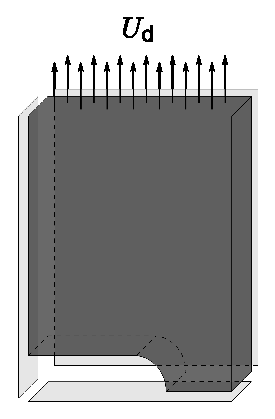
\includegraphics[scale=0.7,clip]{/home/alameddin/phd_thesis/templates/figures/3d_plate_1_8.eps}
\end{figure}
\end{itemize}
}

\frame[t]{\frametitle{Viscoplastic viscodamage material model}
\twocol{\begin{itemize}
		\item State equations\\[0.5cm]
	\end{itemize}
	\begin{equation*}
	\begin{split}
	\fsigma &= (1-D) \ \ffC : \fepse \\
	\fbeta &= \frac{2}{3} \  c \  \falpha \\
	R & = R_\infty \ (1-\mathrm{e}^{-b \ r})\\
	Y & = \frac{1}{2} \  \fepse :  \ffC :  \fepse
	\end{split}
	\end{equation*}}{
	\begin{itemize}
		\item Evolution equations\\[0.5cm]
	\end{itemize}
	\begin{equation*}
	\begin{split}
	\epspdot &= \dot{\lambda} \ \fN\\
	{\dot\falpha} &=\dot{\lambda} \ \left( \z{\fN} - \frac{3 \ a}{2 \ c} \ \fbeta \right)\\
	\dot{r} & = \dot{\lambda}\\
	{\dot{D}} &= \frac{\dot{\lambda}}{1-D} \ {\left( \frac{Y}{S} \right)}^{s} \text{if } (r > p_{\rm D})\\
	\end{split}
	\label{eq:evolution_damage_detailed}
	\end{equation*}}{ }

%\begin{minipage}[t]{0.4\textwidth}
%\begin{itemize}
%{\item }
%\vspace{-0.3cm}
%\begin{equation*}
%\begin{split}
%\fsigma & = \ffC \ \fepse \ (1-D) \\
%\fbeta &= C \ \falpha \\
%Y & = \frac{1}{2} \fepse : \ffC \ \fepse
%\end{split}
%\end{equation*}
%\end{itemize}
%\end{minipage}\hfil\begin{minipage}[t]{0.5\textwidth}
%\begin{itemize}
%{\item Evolution equations}
%\vspace{-0.3cm}
%\small
%\begin{equation*}
%\begin{split}
%{\dot{\epst}}^{\rm p} &=  k \ \vol{\Fp}_+^{n} \ \left[\frac{3}{2} \frac{\ftau}{J_{2}(\ftau)} \right] \frac{1}{1-D}\\
%{\dot\alpha} &= k \ \vol{\Fp}_+^{n} \ \left[ \frac{3}{2} \frac{\ftau}{J_{2}(\ftau)} - \frac{a}{C} \fbeta \right] \\
%{\dot{D}} &=  \kd  \vol{\Fd}_+^{\nd}
%\end{split}
%\end{equation*}
%\end{itemize}
%\end{minipage}
%\vspace{0.5cm}

}

% till here 10 slides

\frame[t]{\frametitle{Model verification}
	\begin{itemize}
		\item With respect to a classical Newton-Raphson scheme \\[0.5cm]
	\end{itemize}
\vfill
\twocol{
\centering
\includegraphics[height=0.55\textheight]{/home/alameddin/phd_thesis/templates/figures/semi_incremental/temporal_scheme_1_1.pdf}
}{
\centering
\includegraphics[height=0.55\textheight]{/home/alameddin/phd_thesis/templates/figures/semi_incremental/temporal_scheme_1_2.pdf}
}{ }
}

\frame[t]{\frametitle{Variable amplitude and frequency loading}
	\begin{itemize}
		\item Amplitudes: $[30,90]\cdot10^{-4}\unit{mm}$ \hfill Time periods: $[20,60]\unit{sec}$\\[0.5cm]
	\end{itemize}
	\vfill
	\twocol{
		\centering
		\includegraphics[height=0.5\textheight]{/home/alameddin/phd_thesis/templates/figures/semi_incremental/temporal_scheme_2_1.pdf}
	}{
		\centering
		\includegraphics[height=0.5\textheight]{/home/alameddin/phd_thesis/templates/figures/semi_incremental/temporal_scheme_2_2.pdf}
	}{
\uncover<2>{\begin{block}{ \centering Number of modes is eight}
\end{block}}}
}

\frame[t]{\frametitle{Random amplitude loading}
	\begin{itemize}
		\item $100$ cycles with different orthonormalisation schemes
	\end{itemize}
	\vfill
	\twocol{
		\centering
		\includegraphics[height=0.5\textheight]{/home/alameddin/phd_thesis/templates/figures/modal_optimisation/mgs_number_of_pgd_modes.pdf}\\
		\qquad \qquad Gram-Schmidt
	}{
		\centering
		\includegraphics[height=0.5\textheight]{/home/alameddin/phd_thesis/templates/figures/modal_optimisation/excessive_svd_m8_number_of_pgd_modes.pdf}\\
		\qquad SVD scheme
	}{ }
}

\frame[t]{\frametitle{Random amplitude loading}
	\begin{itemize}
		\item Required time\\[0.5cm]
	\end{itemize}
	\vfill
	\twocol{
		\centering
		\includegraphics[height=0.5\textheight]{/home/alameddin/phd_thesis/templates/figures/modal_optimisation/temporal_update_timing.pdf}\\
		\hfil Temporal update
	}{
		\centering
		\includegraphics[height=0.5\textheight]{/home/alameddin/phd_thesis/templates/figures/modal_optimisation/orthonormalisation_timing.pdf}\\
		\hfil Orthonormalisation step
	}{ }
}

\frame[t]{\frametitle{Random amplitude loading}
	\begin{itemize}
		\item $10000$ cycles, uniform distribution in $[53,56]\cdot 10^{-2} \unit{mm}$\\[0.5cm]
	\end{itemize}
	\vfill
	\twocol{
		\centering
		\includegraphics[height=0.51\textheight]{/home/alameddin/phd_thesis/templates/figures/semi_incremental/temporal_scheme_3_1.pdf}
	}{
		\centering
		\includegraphics[height=0.5\textheight]{/home/alameddin/phd_thesis/templates/figures/semi_incremental/temporal_scheme_3_2.pdf}
	}{\vspace{-0.5cm}
		\only<2>{
			\begin{itemize}
				\item $D_{\mathrm{c}}=0.3 \hfil \rightarrow \hfil  P_{\mathrm{f}}=5.4\%$
				\item Requirements: $[15-35]\unit{min}$ and $[1-1.5]\unit{GB}$
			\end{itemize}
		}
		\uncover<3>{\begin{block}{ \centering Time-saving factors $50 \sim 100$}
	\end{block}}
}
}

\section{Conclusions and future research}
\begin{frame}{Outline}
\tableofcontents[currentsection]
\end{frame}

\frame{\frametitle{Conclusion and future research}
\vspace{0.5cm}
\begin{itemize}
\item Efficient cycle by cycle simulation for damage problems
\item Open-source: \url{gitlab.com/shadialameddin/romfem}\\[0.3cm]
\vfill
\pause
\textbf{Challenges}
\item The computation of the local stage
\item The integration of the error indicator\\[0.3cm]
\vfill
\pause
\textbf{Future development}
\item PGD of all QoI in the local stage
\item Machine learning to approximate the constitutive manifold
\end{itemize}
\pause
{\begin{block}{ \centering Thank you for your attention}
\end{block}}
}

\frame{\frametitle{The global stage}
	\begin{itemize}
		\item Weak form at iteration $i+1$
		\begin{equation*}
		\hspace{-0.5cm} \footnotesize \intspt \stepk[]{\fsigma}:\feps(\su) \dspt = \intspt \fb \cdot \su  \d \Omega \d t+ \intt{\pOmegaN}  \bar{\ft} \cdot \su \d S \d t, \quad \forall \su \in \cal{U}_{\mathrm{0}}
		\end{equation*}
		\vfill
		\item Correction $\Delta\stepk[]{\bullet}=\stepk[]{\bullet}-\stepi[]{\bullet}$
		\begin{align*}
		& \Delta\stepk[]{\fsigma} - {\ffH^-} \Delta\stepk[]{\feps} - \hf=\fzero, \ \  \hf  = \underbrace{(\stepj{\fsigma}-\stepi{\fsigma}) - {\ffH^-} (\stepj[]{\feps}-\stepi[]{\feps})}_{known} \\
		\intspt & \Delta \stepk[]{\fsigma} : \feps(\Delta \su) \ \d \Omega \d t = 0
		\end{align*}
	\end{itemize}
}

\frame{\frametitle{Proper Generalised Decomposition}
	\begin{itemize}
		\item  Low-rank approximation of the solution
		\begin{equation*}
		{u}(\fx,t)=\ds \sum_{i=1}^{N} \lambda_i(t) \ v_i(\fx)
		\end{equation*}
		\item  Enriching with one mode
		\begin{align*}
		\Delta u = \lambda(t) \ v(\fx) \qquad \Delta u^\ast = \lambda^\ast \ v + \lambda \ v^\ast
		\end{align*}
		\item Updating $(\mu)$ previously generated time modes
		\begin{align*}
		\Delta u = \ds \sum_{i=1}^{\mu} \Delta \lambda_i(t) \ \underbrace{v_i(\fx)}_{known}
		\end{align*}
	\end{itemize}
}

\frame{\frametitle{Static admissibility}
	\footnotesize
	\begin{itemize}
		\item  Static admissibility and global search direction
		\footnotesize{\begin{align*}
			\intspt  {\ffH^-} \Delta\stepk[]{\feps}  : \feps(\Delta \su) \ \d \Omega \d t & = - \intspt \hf : \feps(\Delta \su) \ \d \Omega \d t
			\end{align*}}
		\item Space problem: {\footnotesize $ \tiny \vol{\bullet} = \intT \bullet \ \d t$}, given $\lambda_j$
		\footnotesize{
			\begin{align*}
			\vol{\lambda_j \lambda_j} \intS \grad{v}^\ast  : {\ffH^-}  \grad{v_{j+1}} \ \d \Omega & = - \vol{\lambda_j} \intS \grad{v}^\ast : \hf \d \Omega
			\end{align*}}
		\vspace{-0.2cm}
		\item Time problem, given $v_{j+1}$:
		\begin{align*}
		\footnotesize
		\intT \lambda^\ast \left[ \intS  \grad{v_{j+1}} : {\ffH^-} \ \grad{v_{j+1}} \d \Omega \right] \lambda_{j+1} \ \d t & = - \vol{\lambda^\ast} \intS  \grad{v_{j+1}} : \hf \d \Omega
		\end{align*}
	\end{itemize}
	%		\mediabutton[jsaction={anim.myAnim.playFwd();}]{\fbox{\strut Play}}
	%		\mediabutton[jsaction={anim.myAnim.pause();}]{\fbox{\strut Pause}}
	%		 \includegraphics[width=0.4\linewidth]{./img/lating-0.png}
}

\end{document}
